\documentclass[10pt]{article}

\usepackage[utf8]{inputenc}
\usepackage[T1]{fontenc}
\usepackage{lmodern}
\usepackage{amsmath,amssymb,amsthm}
\usepackage{array,booktabs}
\usepackage[table]{xcolor}
\usepackage{enumitem}
\usepackage{geometry}
\usepackage{algpseudocode}
\usepackage{float}
\usepackage{multicol}
\usepackage[ruled, vlined, algoruled]{algorithm2e} % Options for styling
\usepackage{tikz}
\usetikzlibrary{arrows.meta,positioning}
\usepackage{hyperref}
\geometry{top=0.65in,bottom=0.65in,left=0.2in,right=0.2in}
\hypersetup{
  pdftitle={CS4234: Optimization Algorithms - Midterm Notes},
  pdfauthor={Wxy2003-xy},
  colorlinks=true,
  linkcolor=blue!60!black,
  urlcolor=cyan!50!black,
  linktoc=all
}

\setlength{\multicolsep}{0pt}

\setlist{nosep,leftmargin=*}
\renewcommand{\arraystretch}{1.2}
\newcolumntype{P}[1]{>{\raggedright\arraybackslash}p{#1}}

\theoremstyle{definition}
\newtheorem{definition}{Definition}[section]
\newtheorem{theorem}[definition]{Theorem}
\newtheorem{lemma}[definition]{Lemma}
\newtheorem{remark}[definition]{Remark}
\newtheorem{corollary}[definition]{Corollary}

\newcommand{\OPT}{\operatorname{OPT}}
\newcommand{\ALG}{\operatorname{ALG}}
\newcommand{\poly}{\operatorname{poly}}
\newcommand{\YES}{\textsc{Yes}}
\newcommand{\NO}{\textsc{No}}
\newcommand{\NP}{\mathsf{NP}}
\newcommand{\coNP}{\mathsf{coNP}}
\newcommand{\PTIME}{\mathsf{P}}
\newcommand{\NPC}{\mathsf{NP\text{-}complete}}

% Colours used to separate the three layers of approximation proofs.
\definecolor{algblue}{RGB}{0,82,155}
\definecolor{optred}{RGB}{180,45,45}
\definecolor{bridgepurple}{RGB}{105,55,145}

\title{CS4234: Optimization Algorithms}
\author{@Wxy2003-xy}
\date{}


\setcounter{tocdepth}{2}
\emergencystretch=2em
\allowdisplaybreaks[1]


\begin{document}\maketitle\tableofcontents\clearpage
\begin{multicols*}{2}

\section{Exam Reference and Proof Toolkit}
\label{ref:toolkit}
\subsection{Choose a technique}
\begin{center}
\small
\begin{tabular}{P{0.25\textwidth}P{0.29\textwidth}P{0.35\textwidth}}
\toprule
\textbf{Problem cue} & \textbf{Method} & \textbf{Comparison with OPT}\\
\midrule
Knapsack, one blocked large item & Density prefix or best singleton & Fractional optimum $\le G+v_{\max}$\\
Several nonnegative objectives & Best of component optimizers & $\OPT\le\sum_j f_j(x_j)\le k\ALG$\\
Cost per newly covered element & Greedy weighted set cover & Element prices sum to $\ALG$; each optimal set pays at most $H_n$ times its cost\\
Destroy fixed-size obstructions & Maximal disjoint packing & Each packed obstruction forces a distinct OPT action\\
At most $k$ covering choices per element & LP threshold $1/k$ & Feasible by a covering constraint; cost $\le kLP^*\le k\OPT$\\
Metric travel and parity & MST, Euler tour, matching & MST costs $\le\OPT$; odd-set matching costs $\le\OPT/2$\\
Nonnegative local rewards & Random labels and indicators & $\OPT\le$ total available reward\\
Deterministic guarantee required & Conditional expectation & Choose a branch whose expectation does not decrease\\
Fractional decisions & LP rounding & Per-object bound, weighted sum, relaxation bound\\
Compatibility and quotas & Layered network flow & Integral flow at a specified target value\\
Vertex throughput or disjointness & Split each vertex & Capacity on $v_{\rm in}\to v_{\rm out}$\\
Minimum cut, secondary objective & Integer capacity perturbation & $(m+1)c_e+1$ preserves capacity priority\\
Large numeric DP coordinate & Scale values & Total rounding loss $\le nK$\\
\bottomrule
\end{tabular}
\end{center}

\subsection{What every solution must state}
\begin{enumerate}
\item \textbf{Model and assumptions:} feasible objects, objective direction, nonnegative
weights, metric properties, integrality, and any special graph structure.
\item \textbf{Algorithm:} explicit choices, stopping rule, and the actual output object.
\item \textbf{Feasibility:} why all constraints hold. For a reduction, prove both directions
and explain how to decode the solution.
\item \textbf{Guarantee:} exhibit a lower bound on $\OPT$ for minimization, or an upper
bound for maximization, then write the complete inequality chain.
\item \textbf{Runtime:} construction plus iterations times work per iteration. Numeric
capacity $C$ has $O(\log(C+1))$ bits; polynomial in $C$ need not mean polynomial in input size.
\end{enumerate}

\subsection{Guarantee conventions and relaxation directions}
For $\rho\ge1$, minimization means $\OPT\le\ALG\le\rho\OPT$ and maximization means
$\OPT/\rho\le\ALG\le\OPT$. Equivalently, a maximization algorithm retains a fraction
$\alpha=1/\rho\le1$. State the inequality explicitly when different sources use different
ratio conventions. For randomized algorithms replace $\ALG$ by $\mathbb E[\ALG]$ in the
promised bound; an expectation guarantee is not a guarantee for every run.
\[
\begin{array}{ll}
\text{Minimization relaxation:}&LP^*\le\OPT,\\
\text{Maximization relaxation:}&LP^*\ge\OPT.
\end{array}
\]
These compare \emph{optimal} relaxation values. An arbitrary fractional feasible objective
does not automatically bound the integral optimum in the required direction. When $\OPT=0$,
use inequalities instead of dividing by it.

\subsection{Probability and inequalities used in the course}
\begin{align*}
\mathbb E[\mathbf1_A]&=\Pr[A], &
\mathbb E\!\left[\sum_iw_iX_i\right]&=\sum_iw_i\mathbb E[X_i],\\
\Pr\!\left[\bigcup_i A_i\right]&\le\sum_i\Pr[A_i], &
\Pr[A\mid B]&=\frac{\Pr[A\cap B]}{\Pr[B]}\quad(\Pr[B]>0).
\end{align*}
Linearity and the union bound require no independence. Products of probabilities need
the corresponding independence assumption. For a nonnegative random cost $Z$ and a success
event $A$ of probability $q>0$,
\[
\mathbb E[Z\mid A]=\frac{\mathbb E[Z\mathbf1_A]}q\le\frac{\mathbb E[Z]}q.
\]
Independent trials with success probability $q$ have expected trial count $1/q$ and
failure probability $(1-q)^t$ after $t$ trials. Cost and success within one trial may be correlated.
\begin{align*}
1-x&\le e^{-x}, &
\prod_{i=1}^k a_i&\le\left(\frac1k\sum_{i=1}^k a_i\right)^k\quad(a_i\ge0),\\
\left(\sum_i a_ib_i\right)^2&\le\left(\sum_i a_i^2\right)\left(\sum_i b_i^2\right), &
H_n=\sum_{j=1}^n\frac1j&\le1+\ln n.
\end{align*}
If $g$ is concave on $[0,1]$, then
$g(y)\ge(1-y)g(0)+yg(1)$. In particular, $g(0)=0$ implies $g(y)\ge yg(1)$.
For candidate values, $\max_i A_i\ge\frac1k\sum_i A_i$; this holds pointwise, so it also
holds after taking expectations, without independence between candidates.

\subsection{Small counterexamples and quantifiers to remember}
\begin{itemize}
\item \textbf{Exact equivalence need not preserve approximation:} $q$ disjoint edges plus
an isolated vertex give a maximal-matching cover whose complement has size 1, while
maximum independent set has size $q+1$.
\item \textbf{Maximizing satisfied versus minimizing unsatisfied clauses:} a satisfiable
2-literal clause has optimum unsatisfied count 0, but fair assignment leaves it unsatisfied
with probability $1/4$. A MAX-SAT guarantee does not transfer by subtraction.
\item \textbf{Integral-flow theorem:} an integral maximum flow \emph{exists}; fractional
maximum flows may also exist. Two parallel branches merging before a unit bottleneck can
each carry $1/2$.
\item \textbf{Vertex-cover LP gap:} on $K_n$, $\OPT=n-1$ and $LP^*=n/2$, so the
worst-case gap is at least $2-2/n$. This is not a statement about every $n$-vertex graph.
\item \textbf{Maximal versus maximum:} maximality is enough for the matching-based cover.
Even a maximum matching's endpoints need not form a minimum cover (one edge suffices).
\item \textbf{Numeric versus bit complexity:} $O(mC)$ may be exponential in $\log C$.
Capacity-scaling phases must include threshold 1 for integer capacities.
\end{itemize}



\clearpage\section{Greedy Approximation and Scaling}\label{gre:main}
For each approximation below, feasibility and comparison with an optimal solution are separate proof obligations. Assume nonnegative values and costs, and positive item weights where density is used.

\subsection{Greedy algorithms for 0/1 knapsack}\label{gre:knapsack}
We can relax 0/1 knapsack to fractional knapsack, for which prioritizing items by highest value density is optimal. Applying the same ordering to whole items is a natural first greedy approach, but it can be arbitrarily bad for 0/1 knapsack.

\subsubsection*{Value-density-first greedy}

\begin{algorithm}[H]
  \caption{Value-density-first greedy for 0/1 knapsack}
  \KwIn{
    Values $v_1,\ldots,v_n$, weights $w_1,\ldots,w_n$, capacity $W$
  }
  \KwOut{
    A feasible item set $S_D$ and its total value $V_D$
  }
  $F \gets \{i \in \{1,\ldots,n\}:w_i\leq W\}$\;
  Sort the items in $F$ by non-increasing density $v_i/w_i$\;
  $S_D \gets \varnothing$, $W_D \gets 0$, $V_D \gets 0$\;
  \ForEach{$i \in F$ in density order}{
    \If{$W_D+w_i>W$}{
      \textbf{break}\;
    }
    $S_D \gets S_D\cup\{i\}$\;
    $W_D \gets W_D+w_i$\;
    $V_D \gets V_D+v_i$\;
  }
  \Return $(S_D,V_D)$\;
\end{algorithm}

\subsubsection*{Counterexample}
For an integer capacity $W>2$, consider
\begin{align*}
  v &= \{2, W\}\\
  w &= \{1, W\}
\end{align*}
The value-density-first algorithm takes only the first item and returns value $2$, while the optimal solution takes the second item and returns $W$. 
\[\frac{OPT}{ALG} = \frac{W}{2}\]
There is no constant approximation factor, meaning this algorithm can give an arbitrarily bad result. 
\subsubsection*{Identify the gap}
From the counter example, we can see that a gap is caused by high-value low density (consequently high weight) items. 
This suggests another greedy approach: prioritize items by value rather than by density.


\begin{algorithm}[H]
  \caption{Value-first greedy for 0/1 knapsack}
  \KwIn{
    Values $v_1,\ldots,v_n$, weights $w_1,\ldots,w_n$, capacity $W$
  }
  \KwOut{
    A feasible item set $S_V$ and its total value $V_V$
  }
  $F \gets \{i \in \{1,\ldots,n\}:w_i\leq W\}$\;
  Sort the items in $F$ by non-increasing value $v_i$\;
  $S_V \gets \varnothing$, $W_V \gets 0$, $V_V \gets 0$\;
  \ForEach{$i \in F$ in value order}{
    \If{$W_V+w_i\leq W$}{
      $S_V \gets S_V\cup\{i\}$\;
      $W_V \gets W_V+w_i$\;
      $V_V \gets V_V+v_i$\;
    }
  }
  \Return $(S_V,V_V)$\;
\end{algorithm}

This solves the problem of overlooking a high-value item, but it can still be arbitrarily bad.
\subsubsection*{Counterexample for value-first greedy}
Let the capacity be an integer $W>2$, with one heavy item and $W$ unit items:
\begin{align*}
  v &= \{2, \underbrace{1,1,\ldots,1}_{W\text{ items}}\},\\
  w &= \{W, \underbrace{1,1,\ldots,1}_{W\text{ items}}\}.
\end{align*}
Value-first greedy takes the heavy item, fills the knapsack, and returns value $2$. The optimal solution takes all $W$ unit items and has value $W$. Therefore,
\[
  \frac{OPT}{ALG}=\frac{W}{2}\longrightarrow\infty.
\]
Thus neither density-first nor value-first greedy has a constant approximation factor by itself.

\subsubsection*{Modified greedy: keep the better candidate}
The fractional solution is a whole-item density-greedy prefix plus a fraction of the first item that does not fit. This identifies the two candidates needed for the repair: the density-greedy prefix and the best feasible singleton.


\begin{algorithm}[H]
  \caption{Modified two-candidate greedy for 0/1 knapsack}
  \KwIn{
    Values $v_1,\ldots,v_n$, weights $w_1,\ldots,w_n$, capacity $W$
  }
  \KwOut{
    A feasible item set $S$ and its total value
  }
  $F \gets \{i \in \{1,\ldots,n\}:w_i\leq W\}$\;
  \If{$F=\varnothing$}{
    \Return $(\varnothing,0)$\;
  }
  Sort the items in $F$ by non-increasing density $v_i/w_i$\;
  $S_G \gets \varnothing$, $W_G \gets 0$, $V_G \gets 0$\;
  \ForEach{$i \in F$ in density order}{
    \If{$W_G+w_i>W$}{
      \textbf{break}\;
    }
    $S_G \gets S_G\cup\{i\}$\;
    $W_G \gets W_G+w_i$\;
    $V_G \gets V_G+v_i$\;
  }
  $i_{\max}\gets\arg\max_{i\in F}v_i$\;
  $S_M\gets\{i_{\max}\}$, $V_M\gets v_{i_{\max}}$\;
  \eIf{$V_G\geq V_M$}{
    \Return $(S_G,V_G)$\;
  }{
    \Return $(S_M,V_M)$\;
  }
\end{algorithm}

The value-first greedy solution always contains the best feasible singleton, so it could replace the singleton candidate and would preserve the guarantee. The singleton is used because it is the minimal repair required by the proof.



\subsection{The best-of-candidates argument}
\label{gre:best}
Let $g(x)=\sum_{i=1}^k f_i(x)$ on a common feasible domain, with $f_i(x)\ge0$.
Suppose $x_i$ is a \emph{global} maximizer of $f_i$. Return the candidate $x_j$ with
largest $g(x_j)$. For an optimum $x^*$,
\[
\OPT=\sum_i f_i(x^*)\le\sum_i f_i(x_i)
\le\sum_i g(x_i)\le k\max_i g(x_i)=k\ALG.
\]
Nonnegativity justifies the middle inequality. Feasibility follows because every candidate
lies in the same domain. Evaluate all $k$ candidates in addition to the cost of finding them.

For modified knapsack, the fractional optimum consists of a whole-item density prefix
of value $G$ and at most one fractional item $\theta v_j$, $0\le\theta\le1$. All overweight
items were discarded, so the best feasible singleton has value at least $v_j$. Therefore
\[
\OPT\le\OPT_{\rm frac}=G+\theta v_j\le G+v_{\max}
\le2\max\{G,v_{\max}\}=2\ALG.
\]
If all items fit, the density prefix itself is optimal. Sorting dominates the running time,
$O(n\log n)$.

\subsection{Subset sum and group admission}
\label{gre:subset}
Given positive item sizes $a_i$ and capacity $B$, maximize the admitted total subject to
the capacity. Groups must be accepted in full. Ignore items larger than $B$.

\begin{algorithm}[H]
\caption{Largest-first admission}
\KwIn{Positive sizes $a_1,\ldots,a_n$; fixed capacity $B$}
\KwOut{A feasible index set $S$}
Sort indices in nonincreasing order of $a_i$\;
$S\gets\varnothing$; $A\gets0$\;
\ForEach{index $i$ in that order}{
  \If{$A+a_i\le B$}{$S\gets S\cup\{i\}$; $A\gets A+a_i$\;}
}
\Return $S$\;
\end{algorithm}
\begin{proof}
The admission test preserves $A\le B$. If the final total $A\ge B/2$, then
$A\ge\OPT/2$. Otherwise the final remaining capacity exceeds $B/2$.
There cannot have been a feasible item larger than $B/2$: the first such item in sorted
order would have fitted into the initially empty solution, contradicting $A<B/2$.
Every feasible item is therefore at most $B/2$ and fits whenever considered, because
remaining capacity never falls below its final value. All feasible items were admitted,
so $A=\OPT$. Sorting gives $O(n\log n)$ time.
\end{proof}
\textbf{Tight family:} capacity $2k$, sizes $k+1,k,k$. Greedy returns $k+1$, whereas
$\OPT=2k$; the retained fraction tends to $1/2$.

\paragraph{Read-only array and constant extra space.}
Scan once for a largest individually feasible item, of size $M$. If none exists, return
the empty solution. If $M\ge B/2$, return that item. Otherwise scan again in the original
order, admitting each item when it fits. If the result is below $B/2$, every feasible item
(all smaller than $B/2$) fitted, so it is optimal. Otherwise it is at least $\OPT/2$.
Time is $O(n)$ and extra space is $O(1)$ when admissions can be output as a stream.

\subsection{Knapsack FPTAS: value-indexed dynamic programming}
\label{gre:fptas}
An FPTAS returns a feasible value at least $(1-\epsilon)\OPT$ for $0<\epsilon<1$, with
time polynomial in input length and $1/\epsilon$. Assume positive integer weights and
nonnegative integer values. Discard items with $w_i>W$, redefine $n$ to count the remaining
items, and let $V=\max_i v_i$. If no items remain or $V=0$, return the empty set.

\paragraph{Exact pseudo-polynomial DP.}
For $0\le i\le n$ and $0\le p\le nV$, define
\[
D[i,p]=\text{minimum weight using items }1,\ldots,i\text{ with total value exactly }p.
\]
Set $D[0,0]=0$ and other impossible states to $+\infty$. The recurrence is
\[
D[i,p]=
\begin{cases}
\min\{D[i-1,p],\ w_i+D[i-1,p-v_i]\},&p\ge v_i,\\
D[i-1,p],&p<v_i.
\end{cases}
\]
Compute rows in increasing $i$. Return the largest $p$ with $D[n,p]\le W$, and backtrack
through minimizing choices to recover its subset. Every optimum either omits item $i$ or
contains it, leaving value $p-v_i$ among earlier items; conversely both recurrence alternatives
describe valid subsets. This proves the state invariant by induction. There are $O(n^2V)$
states and constant work per state, giving $O(n^2V)$ time and space. Two rows give $O(nV)$
space when only the optimum value is needed.

\paragraph{Scale the value coordinate, not the weights.}
Set $K=\epsilon V/n$ and $\hat v_i=\lfloor v_i/K\rfloor$. Run the value-indexed DP using
$\hat v_i$ and the unchanged weights. Since $\hat v_i\le n/\epsilon$, the total scaled
value is at most $n^2/\epsilon$ and the runtime is $O(n^3/\epsilon)$ arithmetic operations.
Weights and arithmetic are represented with polynomially many bits; rational $\epsilon$
can be handled by integer arithmetic in $\lfloor nv_i/(\epsilon V)\rfloor$.

\begin{proof}[Approximation guarantee]
Let $S$ maximize scaled value and let $S^*$ be an original optimum. For each item,
$K\hat v_i\le v_i<K(\hat v_i+1)$. Feasibility is unchanged because weights were not rounded.
Writing $v(S)=\sum_{i\in S}v_i$ and similarly for $\hat v(S)$,
\begin{align*}
v(S)&\ge K\hat v(S)\ge K\hat v(S^*)\\
&\ge v(S^*)-K|S^*|\ge\OPT-nK\\
&=\OPT-\epsilon V\ge(1-\epsilon)\OPT.
\end{align*}
The last step uses $V\le\OPT$: the largest remaining item fits by itself. This is why
overweight items must be discarded \emph{before} defining $V$.
\end{proof}
Scaling values does not reduce the state space of a weight-indexed $O(nW)$ DP. Neither
$V$ nor $W$ is a constant; the improvement comes from bounding the scaled coordinate.



\subsection{Weighted set cover: greedy charging}\label{gre:setcover}
Given a universe $U$ and a family of candidate sets $\mathcal{S}_U$, each
$S\in\mathcal{S}_U$ has a non-negative cost $\operatorname{cost}(S)$. The
weighted set cover problem asks for a subfamily $S'\subseteq\mathcal{S}_U$
such that
\[
  \bigcup_{S\in S'}S=U,
\]
while minimizing $\sum_{S\in S'}\operatorname{cost}(S)$.

\subsubsection*{Greedy score}
Let $R$ be the set of elements that remain uncovered. For every set that can
still cover at least one new element, define
\[
  \operatorname{score}(S)=
  \frac{\operatorname{cost}(S)}{|S\cap R|}.
\]
This is the average cost per newly covered element. Greedy repeatedly chooses
a set of minimum score.


\begin{algorithm}[H]
\KwIn{Universe $U$, candidate family $\mathcal{S}_U$ with costs}
\KwOut{A set cover $S'\subseteq\mathcal{S}_U$}
$R\gets U$ and $S'\gets\emptyset$\;
\While{$R\neq\emptyset$}{
  $A_i\gets\displaystyle
  \arg\min_{\substack{S\in\mathcal{S}_U\\S\cap R\neq\emptyset}}
  \dfrac{\operatorname{cost}(S)}{|S\cap R|}$\;
  $S'\gets S'\cup\{A_i\}$\;
  $R\gets R\setminus A_i$\;
}
\Return{$S'$}\;
\end{algorithm}

We prove
\[
  \ALG\leq H_n\OPT\leq(1+\ln n)\OPT,
  \qquad
  H_n=\sum_{j=1}^{n}\frac1j,\qquad n=|U|.
\]

\begin{proof}
Assume the instance is feasible, so
$\bigcup_{S\in\mathcal{S}_U}S=U$. The invariant is
\[
  U\setminus R=\bigcup_{A\in S'}A:
\]
the elements removed from $R$ are exactly those covered by the sets already
selected. If $R\neq\emptyset$, feasibility guarantees a candidate set with
$S\cap R\neq\emptyset$, so every iteration removes at least one element from
$R$. Hence the algorithm terminates with $R=\emptyset$ and $S'$ is a cover.

\medskip
\noindent
\textcolor{algblue}{\textbf{Blue: express the greedy cost exactly.}}\quad
\textcolor{optred}{\textbf{Red: bound prices using OPT.}}\quad
\textcolor{bridgepurple}{\textbf{Purple: combine the two.}}

\subsubsection*{\textcolor{algblue}{1. Rewrite the greedy cost as element prices}}

Let $R_i$ be the set of uncovered elements at the beginning of iteration $i$,
and let $A_i$ be the set selected in that iteration. The elements newly
covered in this iteration are exactly $A_i\cap R_i$. For each
$e\in A_i\cap R_i$, define
\[
  \color{algblue}
  p(e)=\frac{\operatorname{cost}(A_i)}{|A_i\cap R_i|}.
\]
This is an accounting price, not an intrinsic cost of $e$. Already-covered
elements of $A_i$ are not charged again. The prices assigned in iteration
$i$ recover exactly the cost of $A_i$:
\[
  \color{algblue}
  \sum_{e\in A_i\cap R_i}p(e)
  =|A_i\cap R_i|\frac{\operatorname{cost}(A_i)}{|A_i\cap R_i|}
  =\operatorname{cost}(A_i).
\]
Every element is newly covered exactly once, so summing over all iterations
gives the exact identity
\[
  \color{algblue}
  \boxed{\ALG=\sum_{A\in S'}\operatorname{cost}(A)
  =\sum_{e\in U}p(e).}
\]

\subsubsection*{\textcolor{optred}{2. Use one optimal set to bound its elements' prices}}

Let $\mathcal{O}\subseteq\mathcal{S}_U$ be a fixed optimal cover and define
\[
  \color{optred}
  \OPT=\sum_{S\in\mathcal{O}}\operatorname{cost}(S).
\]
Fix any one set $S^*\in\mathcal{O}$ and let $m=|S^*|$. The set $S^*$ may or
may not also be selected by greedy; the proof only needs it to be an available
candidate for comparison.

Order its elements by when greedy first covers them:
\[
  S^*=\{e_1,e_2,\ldots,e_m\}.
\]
If several elements are first covered in the same iteration, break the tie
arbitrarily. Let $j(t)$ be the iteration in which $e_t$ is first covered and
define
\[
  r_t=|S^*\cap R_{j(t)}|.
\]
Immediately before that iteration, at least
$e_t,e_{t+1},\ldots,e_m$ are still uncovered. Therefore
\[
  r_t\geq m-t+1.
\]
At iteration $j(t)$, greedy chooses $A_{j(t)}$ with minimum score. Comparing
its score with the available candidate $S^*$ gives
\[
  \color{optred}
  \begin{aligned}
  p(e_t)
  &=\frac{\operatorname{cost}(A_{j(t)})}
          {|A_{j(t)}\cap R_{j(t)}|}\\
  &\leq\frac{\operatorname{cost}(S^*)}{|S^*\cap R_{j(t)}|}
   =\frac{\operatorname{cost}(S^*)}{r_t}\\
  &\leq\frac{\operatorname{cost}(S^*)}{m-t+1}.
  \end{aligned}
\]
The same inequality handles simultaneous coverage: tied elements are all
still in $R_{j(t)}$ before that iteration, making $r_t$ larger and the bound
only stronger. Summing over the elements of this one optimal set,
\[
  \color{optred}
  \begin{aligned}
  \sum_{e\in S^*}p(e)
  &=\sum_{t=1}^{m}p(e_t)\\
  &\leq\operatorname{cost}(S^*)
    \sum_{t=1}^{m}\frac1{m-t+1}\\
  &=\operatorname{cost}(S^*)H_m
   \leq\operatorname{cost}(S^*)H_n.
  \end{aligned}
\]
This is a bound on the \emph{accounting prices of elements in $S^*$}; it is
not a separate cost paid by greedy to cover only those elements.

\subsubsection*{\textcolor{bridgepurple}{3. Bridge the optimal-set bounds back to ALG}}

Every $e\in U$ belongs to at least one set in the optimal cover $\mathcal O$.
Thus the middle sum below counts every $p(e)$ at least once (and may count it
more than once when optimal sets overlap):
\[
  \color{bridgepurple}
  \begin{aligned}
  \ALG
  &=\sum_{e\in U}p(e)\\
  &\leq\sum_{S^*\in\mathcal O}\sum_{e\in S^*}p(e)\\
  &\leq\sum_{S^*\in\mathcal O}
      H_n\operatorname{cost}(S^*)\\
  &=H_n\OPT.
  \end{aligned}
\]
Therefore greedy weighted set cover is an $H_n$-approximation, and since
$H_n\leq1+\ln n$, it is also a $(1+\ln n)$-approximation.
\end{proof}



\paragraph{Running time.}
Each iteration covers at least one new element, so there are at most $n=|U|$ iterations.
If $m$ candidate sets are represented by their incidence matrix, recomputing all marginal
scores costs $O(mn)$ per iteration, for $O(mn^2)$ time. Faster updates are possible, but this
already establishes polynomial time. If $U$ is empty, return the empty cover.


\subsection{Vertex cover from a maximal matching}
\label{gre:vc}
View each edge as an element and each vertex as the set of its incident edges. Every
element then belongs to exactly two sets. For the \emph{unweighted} problem, greedily
construct any maximal matching $M$ and return the set $C$ of \textbf{all endpoints of $M$}.

\begin{algorithm}[H]
\caption{Maximal-matching vertex cover}
\KwIn{Undirected graph $G=(V,E)$}
\KwOut{A vertex cover $C\subseteq V$}
$M\gets\varnothing$; mark all vertices unmatched\;
\ForEach{$\{u,v\}\in E$}{
  \If{both $u$ and $v$ are unmatched}{
    $M\gets M\cup\{\{u,v\}\}$; mark $u,v$ matched\;
  }
}
\Return $C=\bigcup_{e\in M}e$\;
\end{algorithm}
\begin{proof}
An uncovered edge would have two unmatched endpoints and could be added to $M$, contrary
to maximality. Any vertex cover must take a distinct endpoint from each pairwise disjoint
matching edge, so $|M|\le\OPT$. Hence $|C|=2|M|\le2\OPT$.
The scan takes $O(|V|+|E|)$ time. Maximum matching is unnecessary; maximality proves
coverage, while disjointness proves the lower bound.
\end{proof}
This unweighted cardinality proof does not give a weighted-vertex-cover guarantee by
simply summing endpoint weights; use LP rounding for that version.

\paragraph{Why complements do not preserve approximation.}
The complement of any vertex cover is an independent set, and $\OPT_{IS}=|V|-\OPT_{VC}$.
But $|C|\le2\OPT_{VC}$ only implies
$|V\setminus C|\ge2\OPT_{IS}-|V|$, which can be useless. On $q$ disjoint edges plus one
isolated vertex, the matching algorithm selects all $2q$ nonisolated vertices. Its complement
has size 1, while $\OPT_{IS}=q+1$. Thus exact optimization equivalence does not imply
approximation preservation.

\subsection{Triangle deletion and disjoint-obstruction packing}
\label{gre:triangles}
To delete as few edges as possible so that an undirected graph becomes triangle-free,
repeatedly find a remaining triangle and delete \emph{all three} of its edges. Return the
union $F$ of deleted edges.
\begin{proof}
The process stops with no triangle. The selected triangles are pairwise edge-disjoint,
because earlier selected edges were deleted. If $k$ triangles were selected, every feasible
deletion set must remove at least one distinct edge from each of these triangles, so
$\OPT\ge k$. Our output has $|F|=3k\le3\OPT$.
One implementation scans all vertex triples once with an adjacency matrix: select a
triangle only if none of its edges was selected earlier. At the end, any surviving triangle
would have been eligible when its triple was scanned, a contradiction. Time is
$O(|V|^3+|E|)$ with constant-time edge tests.
\end{proof}
\textbf{Counterexample to deleting an arbitrary single edge per triangle:}
take a shared edge $ab$ and vertices $v_1,\ldots,v_q$, each joined to both $a$ and $b$.
Deleting $ab$ solves the instance, while repeatedly deleting a spoke can require $q$ edges.

\paragraph{Reusable generalization.}
For fixed forbidden subgraphs whose occurrences cannot be created by deleting edges,
suppose every forbidden configuration has $r$ edges for a fixed constant $r$. Select a maximal
collection of edge-disjoint configurations and delete all their edges. Maximality gives
feasibility, disjointness gives $\OPT\ge k$, and $\ALG=rk\le r\OPT$. Detection must be
polynomial; the fact that $r$ is fixed is relevant. Induced patterns need separate care:
edge deletion can create a new induced pattern. Weighted deletions need a different cost argument.

\paragraph{Greedy by number of triangles removed.}
This is weighted set cover on the universe of original triangles, with each graph edge
covering the triangles that contain it. Recompute marginal coverage after each deletion.
The generic proof gives an $H_N$ bound, where $N$ is the number of original triangles;
it does not by itself establish the factor 3 above.


\clearpage

\section{Metric TSP and Eulerian Structure}\label{tsp:main}

\subsection{General TSP, metric TSP, and the shortcut rule}
The traveling salesperson problem asks for a minimum-cost Hamiltonian
cycle: visit every vertex exactly once and return to the start.  Throughout
the approximation algorithms below, the input is a complete undirected
graph with nonnegative symmetric costs satisfying the triangle inequality
\[
c(u,w)\le c(u,v)+c(v,w).
\]
These are \emph{metric} costs.  Completeness supplies each shortcut edge;
triangle inequality ensures that shortcutting a walk never increases its
cost.  Repeatedly bypass already visited vertices, retaining the final
return to the start, to turn a spanning closed walk into a Hamiltonian cycle.

\paragraph{Why the metric assumption matters.}
General TSP has no polynomial-time approximation with any fixed finite
factor $\rho\ge1$, unless $\PTIME=\NP$.  Reduce Hamiltonian Cycle on an
unweighted graph $G$ with $n$ vertices: complete the graph, give original
edges cost $1$ and nonedges cost an integer $B>\rho n$.  A YES instance has
$\OPT=n$, so a $\rho$-approximation returns cost at most $\rho n$.  In a NO
instance every tour uses a nonedge, hence has cost at least $B>\rho n$.
The algorithm would distinguish the two cases in polynomial time.  For
fixed $\rho$, $B$ has polynomial encoding length.  These constructed costs
need not satisfy triangle inequality; a cost-$B$ shortcut can replace a
two-edge detour of cost $2$.

Metric TSP remains NP-hard: assign costs $1$ to edges of a Hamiltonian Cycle
instance and $2$ to nonedges.  Every triangle satisfies the metric inequality,
and a tour of cost $n$ exists exactly when the original graph is Hamiltonian.
This proves exact hardness, not the absence of constant-factor approximation.

\subsection{Euler circuits, open trails, and orientation}\label{tsp:euler}
An Euler trail uses every \emph{edge occurrence} exactly once; vertices may
repeat.  Parallel edges are distinct occurrences.  An Euler circuit is a
closed Euler trail.  A Hamiltonian cycle instead visits every vertex once.

\begin{theorem}[Euler's criterion]
An undirected multigraph with at least one edge has an Euler circuit iff
all its nonisolated vertices are connected and every vertex has even degree.
It has an Euler trail between distinct vertices $s,t$ iff all nonisolated
vertices are connected and precisely $s,t$ have odd degree.
\end{theorem}
\begin{proof}
In a closed traversal, each arrival at a vertex is paired with a departure,
so every degree is even.  For an open traversal only the start and end have
one unpaired incident edge.

Conversely, start at any nonisolated vertex and keep following unused edges.
An even-degree vertex other than the start cannot be the first place where
this trail gets stuck: after arriving, an unused departure remains.  Thus
the trail closes.  If edges remain, connectivity gives a vertex of the
current circuit incident to unused edges.  The unused-edge degrees are
still even, so construct another closed trail there and splice it into the
first.  Repeat until every edge is used (Hierholzer's algorithm).
For the open case add one extra $\{s,t\}$ edge, find an Euler circuit,
rotate it to place that edge last, and delete the extra edge.
\end{proof}
Using adjacency lists and marking each edge occurrence, Hierholzer's
algorithm runs in $O(|V|+|E|)$ time.  The handshaking identity
$\sum_v\deg(v)=2|E|$ also shows that the number of odd-degree vertices is
even.  Adding one edge toggles the parity of its two endpoints.

\paragraph{Orienting an even-degree connected graph.}
Find an Euler circuit and orient each edge in the direction in which the
circuit traverses it.  The resulting directed graph is strongly connected:
from any vertex $u$, follow the directed circuit cyclically until any desired
vertex $v$ is reached.  Also $\deg^+(v)=\deg^-(v)$ at every vertex.
This proof concerns the nonisolated vertices; a disconnected even-degree
graph does not become strongly connected by orienting its components.

\subsection{Double-tree: a 2-approximation}\label{tsp:doubletree}
\begin{enumerate}
  \item Compute a minimum spanning tree $T$.
  \item Duplicate every edge of $T$, retaining both copies in a multigraph.
  \item Find an Euler circuit in this connected even-degree multigraph.
  \item Shortcut repeated vertex visits to obtain the output tour $H$.
\end{enumerate}
\textbf{Feasibility.} Doubling makes every degree even; the spanning tree
ensures connectivity.  The Euler circuit visits all vertices, and
shortcutting yields a Hamiltonian cycle in the complete graph.

\textbf{Lower bound and guarantee.} Deleting any edge of an optimal tour
leaves a spanning tree, so $c(T)\le\OPT$.  Therefore
\[
\boxed{\ c(H)\le 2c(T)\le2\OPT.\ }
\]
The first inequality uses triangle inequality; the second uses the MST lower
bound.  Dense Prim takes $O(n^2)$ time on the complete graph; doubling,
Euler traversal, and shortcutting take $O(n)$ further time.

\paragraph{Four-vertex metric counterexample to optimality.}
Use the shortest-path metric of the unit-cost cycle $A,B,D,C,A$:
\[
\begin{array}{c|rrrr}
c & A&B&C&D\\\hline
A&0&1&1&2\\
B&1&0&2&1\\
C&1&2&0&1\\
D&2&1&1&0
\end{array}
\]
The tree $\{AB,AC,CD\}$ is an MST of cost $3$.  The doubled tree admits
Euler circuit $A,B,A,C,D,C,A$.  First-visit shortcutting gives
$A,B,C,D,A$, of cost $1+2+1+2=6$.  The original cycle has cost $4$ and is
optimal because every tour has four edges, each of cost at least $1$.
Thus a valid double-tree execution need not be optimal, even on a metric.

\subsection{Christofides: a \texorpdfstring{$3/2$}{3/2}-approximation}\label{tsp:christofides}
\begin{enumerate}
  \item Compute an MST $T$, and let $O=\{v:\deg_T(v)\text{ is odd}\}$.
  \item Find a \emph{minimum-weight perfect matching} $M$ on the complete
        graph induced by $O$, using the original metric costs.
  \item Form the multigraph $T\cup M$, find an Euler circuit, and shortcut
        repeated vertices to produce a tour $H$.
\end{enumerate}
\textbf{Feasibility.} The set $O$ has even cardinality.  Every vertex in
$O$ gains exactly one incident matching edge and becomes even; all other
degrees stay even.  The tree ensures connectivity.  Keep parallel copies
if a matching edge is also in $T$.

\begin{lemma}[Matching budget]
The matching chosen above has cost $c(M)\le\OPT/2$.
\end{lemma}
\begin{proof}
Take an optimal tour and shortcut it to retain only the vertices of $O$.
The resulting even-length cyclic walk has cost at most $\OPT$.  Its
alternating edges split into two perfect matchings $M_1,M_2$ on $O$.
Therefore, by minimum weight of $M$,
\[
c(M)\le\min\{c(M_1),c(M_2)\}
\le\frac{c(M_1)+c(M_2)}2\le\frac{\OPT}2.
\]
If $O$ has two vertices, the restricted cyclic walk traverses their edge
twice; its two edge occurrences give the same one-edge matching.  If
$O=\varnothing$, use the empty matching.
\end{proof}
Combining the spanning and matching budgets with metric shortcutting gives
\[
\boxed{\ c(H)\le c(T)+c(M)\le\OPT+\tfrac12\OPT
       =\tfrac32\OPT.\ }
\]
All steps are polynomial time; minimum-weight perfect matching is the main
additional subroutine beyond double-tree.  A maximal matching is insufficient:
it may leave odd vertices unmatched, and an arbitrary perfect matching has
no $\OPT/2$ cost guarantee.

\subsection{Held--Karp exact dynamic programming}\label{tsp:heldkarp}
This exact algorithm works for arbitrary tour costs; triangle inequality
is unnecessary.  Fix a root $r$.  For $r\in S\subseteq V$ and $v\in S$,
let $D[S,v]$ be the minimum cost of a path starting at $r$, ending at $v$,
and visiting exactly the vertices in $S$, once each.

\textbf{Bases.} $D[\{r\},r]=0$.  Set all impossible states to $\infty$,
including $D[S,r]$ for $|S|>1$ and states with $r\notin S$ or $v\notin S$.
For $v\ne r$,
\[
\boxed{\ D[S,v]=\min_{u\in S\setminus\{v\}}
        \bigl(D[S\setminus\{v\},u]+c(u,v)\bigr).\ }
\]
\textbf{Why the recurrence is exact.} The penultimate vertex $u$ partitions
all feasible paths.  Removing their last edge leaves precisely a feasible
path for the smaller state; conversely, appending $(u,v)$ to any such path
gives a feasible path for $(S,v)$.

Evaluate states in increasing $|S|$.  For $n\ge2$, close the path by returning
to $r$:
\[
\OPT=\min_{v\ne r}\bigl(D[V,v]+c(v,r)\bigr).
\]
Store a minimizing predecessor with each state; choose the minimizing final
vertex, backtrack while removing the last vertex from $S$, reverse the
resulting sequence, and append $r$.  There are $O(n2^n)$ states with $O(n)$
transitions each, giving $O(n^2 2^n)$ time and $O(n2^n)$ space, including
predecessors.  This is exponential, although faster than enumerating tours.


\clearpage

\section{Randomization and Derandomization}\label{ra:main}

\subsection{The indicator-variable proof template}
For a maximization objective with nonnegative local rewards, write
\[
  \ALG=\sum_i w_i I_i,\qquad
  \mathbb E[\ALG]=\sum_i w_i\Pr[I_i=1].
\]
Linearity of expectation does \emph{not} require the indicators to be
independent. Independence is needed only when a probability calculation
multiplies probabilities of separate random choices. If every reward is
collected with probability at least $\alpha$ and
$W=\sum_iw_i\ge\OPT$, then $\mathbb E[\ALG]\ge\alpha\OPT$.
This guarantees the existence of a good outcome, not that every run is good.
An expected approximation bound alone is not a high-probability bound.

\subsection{Weighted MAX-CUT, MAX-\texorpdfstring{$k$}{k}-CUT, and MAX-DICUT}
Assume nonnegative edge weights and remove self-loops, which can never cross
a cut. For undirected MAX-$k$-CUT, independently label every vertex uniformly
from $\{1,\ldots,k\}$, for $k\ge2$. Count edges whose endpoint labels differ.
For every edge $e=\{u,v\}$,
\[
  \Pr[I_e=1]=1-\sum_{a=1}^k\Pr[u=a,v=a]=1-\frac1k.
\]
Consequently
\[
  \mathbb E[\ALG]=(1-1/k)W\ge(1-1/k)\OPT.
\]
The ordinary MAX-CUT case is $k=2$, giving $\OPT/2$; MAX-3-CUT gives
$2\OPT/3$. A run takes $O(n+m)$ time including evaluation.

For directed MAX-DICUT, select each vertex into $S$ independently with
probability $1/2$, and count only arcs from $S$ to $V\setminus S$.
Each arc $(u,v)$ is counted with probability $1/4$, so
$\mathbb E[\ALG]=W/4\ge\OPT/4$.
Do not count arcs in both directions: doing so changes the objective.
LP rounding improves the retained fraction to $1/2$
(Section~\ref{lp:dicut}).

\subsection{Conditional expectation: how to remove randomness}\label{ra:conditional}
Let $F$ be the expected final objective conditional on the decisions already
fixed. If the next random variable has outcomes $a$ with probabilities $p_a$,
then
\[
  F=\sum_a p_a F_a,\qquad
  F_a=\mathbb E[\ALG\mid\text{fixed decisions},X=a].
\]
At least one positive-probability branch has $F_a\ge F$. Fix such a branch and
repeat. The invariant is that the conditional expectation never decreases;
after the last decision it equals the actual objective. Thus the deterministic
output is at least the initial expectation. To claim a polynomial-time
algorithm, show how to compute each $F_a$ in polynomial time.

\subsubsection*{MAX-$k$-CUT: computable conditional contributions}
Under a partial labelling, an edge with both endpoints fixed contributes its
full weight if their labels differ and zero otherwise. An edge with at least
one endpoint unfixed contributes $(1-1/k)w_e$. When assigning a vertex $v$,
only edges to already fixed neighbors have label-dependent contributions.
Choose a label $a$ maximizing
\[
  \sum_{u:\{u,v\}\in E,\;u\text{ fixed},\;\operatorname{label}(u)\ne a}w_{uv},
\]
equivalently minimizing the weight of fixed neighbors with label $a$.
Process vertices in any order. If $k\ge n$, assign distinct labels to all
vertices instead; this cuts every edge and is optimal. For $k<n$, the
conditional-expectation procedure gives a deterministic
$(1-1/k)$ retained-value approximation in $O(m+nk)$ time by accumulating
neighbor weights in $k$ buckets at each vertex.

\textbf{Worked MAX-CUT example.}
For a unit-weight triangle the initial expectation is $3/2$. Fix the first
vertex to side 0; the expectation remains $3/2$. Putting the second on side 1
makes their edge contribute 1 and the two unresolved edges contribute $1/2$
each, giving conditional expectation 2. Either choice for the third vertex
then yields cut value 2.

\subsubsection*{MAX-SAT: computable conditional contributions}
First remove duplicate literals, discard empty clauses (always false), and
separate tautologies (always true). Thus every remaining clause contains
distinct variables and no variable together with its negation. Suppose an
unfixed variable $x_j$ is independently true with probability $p_j$.
For each clause $C_i$, its conditional expected contribution is
\[
  \begin{cases}
    w_i, &\text{a fixed literal is already true},\\
    0, &\text{all literals are fixed and false},\\
    w_i\left(1-\displaystyle\prod_{\ell\text{ unfixed in }C_i}
       q_\ell\right), &\text{otherwise},
  \end{cases}
\]
where $q_{x_j}=1-p_j$ and $q_{\neg x_j}=p_j$ are literal-failure
probabilities. For fair variables and $r$ unfixed literals, the last line is
$w_i(1-2^{-r})$. Evaluate the total for setting the next variable to 0 and
to 1, and keep the larger value. Scanning all $L$ literal occurrences for
each of $n$ variables gives $O(nL)$ arithmetic operations. This works for
fair, biased, and LP-derived independent probabilities.

\textbf{Worked example.}
For unit-weight clauses $(x)$ and $(\neg x\lor y)$ with fair variables,
$F=1/2+3/4=5/4$. Setting $x=1$ gives $F_1=1+1/2=3/2$; setting $x=0$
gives $F_0=0+1=1$. Choose $x=1$, then $y=1$, obtaining value 2.

For a directed cut with arbitrary independent membership probabilities,
an arc's conditional contribution is $w_{uv}p'_u(1-p'_v)$, where $p'_v$ is
0 or 1 for a fixed vertex and its original probability otherwise.
This also makes both MAX-DICUT rounding schemes below derandomizable.

\subsection{Weighted MAX-SAT by fair and biased assignment}\label{ra:sat}
Use the clause preprocessing above; handle tautological clauses as a constant
reward added to every solution. All weights are nonnegative. In this
subsection and Section~\ref{lp:sat}, $W$, $\OPT$, and $LP^*$ refer to the
remaining formula after removing constant clauses. If the removed true
clauses have total weight $T\ge0$, restore it at the end:
$\ALG_{\rm total}=T+\ALG$ and $\OPT_{\rm total}=T+\OPT$.
Every retained-fraction guarantee $\ALG\ge\alpha\OPT$ with $0\le\alpha\le1$
(also in expectation) is preserved because
$T+\alpha\OPT\ge\alpha(T+\OPT)$.
For a remaining
clause $C_i$ of length $\ell_i\ge1$, fair independent assignment gives
\[
  \Pr[C_i\text{ satisfied}]=1-2^{-\ell_i},\qquad
  \mathbb E[\ALG]=\sum_iw_i(1-2^{-\ell_i})\ge W/2\ge\OPT/2.
\]
The satisfaction probability \emph{increases} with clause length. If every
clause has at least $k$ literals, the guarantee strengthens to
$(1-2^{-k})\OPT$. An assignment and its value can be computed in $O(n+L)$
time, where $L$ is the number of literal occurrences.

\subsubsection*{Biased assignment and the unit-clause issue}
Merge repeated unit clauses by adding their weights. For each variable,
rename it consistently throughout the formula if needed so that the total
positive unit-clause weight is at least the negative one. Let $N$ be the sum
of the negative unit-clause weights after this renaming. Every assignment
loses at least the smaller weight in each opposing pair, so
$\OPT\le W-N$.

Set every renamed variable independently true with probability
$p\in[1/2,1]$. A clause with $a$ positive and $b$ negative literals is
satisfied with probability
\[
  1-(1-p)^a p^b\ge1-p^{a+b}.
\]
In a lower bound, ignore the negative unit clauses. Every remaining unit
clause is satisfied with probability $p$, and every nonunit clause with
probability at least $1-p^2$. Therefore
\[
  \mathbb E[\ALG]\ge\min\{p,1-p^2\}(W-N)
    \ge\min\{p,1-p^2\}\OPT.
\]
The maximum occurs when $p=1-p^2$, giving
\[
  p=\frac{\sqrt5-1}{2},\qquad
  \mathbb E[\ALG]\ge\frac{\sqrt5-1}{2}\OPT.
\]
If no negative unit clauses remain, this simplifies to $N=0$.
Without the renaming/upper-bound argument, assuming all unit clauses are
positive is not justified. Conditional expectation gives deterministic
versions of these guarantees.

\section{Linear Programming and Rounding}\label{lp:main}

\subsection{Modelling, relaxation, and the direction of the bound}\label{lp:template}
An ILP uses integer variables; a $0$--$1$ formulation uses binary decision
variables. A relaxation replaces $x\in\{0,1\}$ by $0\le x\le1$ and keeps
the linear constraints. Its feasible set contains all integral feasible
points. Write $LP^*$ for the \emph{optimal} relaxed objective:
\[
  \begin{array}{c|c|c}
    &\text{relaxation bound}&\text{target rounding proof}\\\hline
    \text{minimization}&LP^*\le\OPT&\ALG\le\rho LP^*\le\rho\OPT\\
    \text{maximization}&LP^*\ge\OPT&
       \mathbb E[\ALG]\ge\alpha LP^*\ge\alpha\OPT
  \end{array}
\]
An arbitrary feasible fractional objective is not necessarily a valid bound
on $\OPT$ in the displayed direction. LP is solvable in polynomial time in
its encoding length; general ILP is NP-hard. After rounding, prove
\emph{feasibility} separately from the objective bound.

\textbf{Proving a model is exact.}
Show both (i) each original solution gives a feasible integral point of the
same objective and (ii) an integral point decodes into a solution of at least
its objective for maximization (at most for minimization). These establish
equality of optimal values. An auxiliary reward variable often needs only
upper bounds: maximizing a nonnegative weighted objective pushes it up when
possible. Such constraints need not force its intended Boolean meaning at
\emph{every feasible point}. If its coefficient is zero, it need not be
pushed up even at an optimum; the decoded solution and optimal value remain
correct. Add equivalence constraints if the variable's exact meaning is
required independently of the objective.

\subsection{Weighted vertex cover: threshold rounding}\label{lp:vc}
For nonnegative vertex costs $c_v$, let $x_v$ indicate selection. The ILP is
\[
  \min\sum_{v\in V}c_vx_v
  \quad\text{subject to}\quad
  x_u+x_v\ge1\quad(\{u,v\}\in E),\qquad x_v\in\{0,1\}.
\]
Relax to $[0,1]$, obtain an optimum $x^*$, and return
$C=\{v:x_v^*\ge1/2\}$. At least one endpoint of every edge reaches $1/2$,
so $C$ is feasible. Also
\[
  c(C)=\sum_{v\in C}c_v
    \le\sum_{v\in C}2c_vx_v^*
    \le2LP^*\le2\OPT.
\]
The algorithm is polynomial time (LP plus a linear scan).
On the unweighted complete graph $K_n$, $\OPT=n-1$ and $LP^*=n/2$:
the all-$1/2$ point is feasible, and summing all edge constraints gives
$(n-1)\sum_vx_v\ge n(n-1)/2$. Hence the worst-case integrality gap is
at least $2-2/n$, approaching 2. This is a family of gap examples, not a
claim that every $n$-vertex graph has this gap.

\subsection{Set cover: bounded frequency}\label{lp:cover}
Let $U$ be a universe, $S_1,\ldots,S_m$ candidate sets with
$\bigcup_jS_j=U$, and costs $c_j\ge0$. One binary variable per set suffices:
\[
  \min\sum_{j=1}^m c_jx_j
  \quad\text{subject to}\quad
  \sum_{j:e\in S_j}x_j\ge1\quad(e\in U),\qquad x_j\in\{0,1\}.
\]
There is no need for an extra variable indicating coverage when every
element must be covered. If each element belongs to at most $k$ sets,
relax and select every set with $x_j^*\ge1/k$. Each covering constraint has
at most $k$ terms, so at least one reaches the threshold. The cost satisfies
\[
  \ALG\le k\sum_jc_jx_j^*=kLP^*\le k\OPT.
\]
This generalizes vertex-cover rounding, where an edge has two endpoint
choices. The hypothesis is bounded \emph{frequency}, not bounded set size.
For example, with one element and two identical cost-1 singleton sets,
$(1/2,1/2)$ is LP-optimal. Each set has size 1, but threshold 1 selects
nothing. This disproves the corresponding threshold proof for bounded set
size.

\subsection{Weighted MAX-SAT: LP rounding}\label{lp:sat}
For the preprocessed formula of Section~\ref{ra:sat}, use $x_j$ for a
variable's truth value and $y_i$ for the reward of clause $C_i$:
\[
  \begin{aligned}
    \max\quad &\sum_iw_i y_i\\
    \text{subject to}\quad &
      y_i\le\sum_{x_j\in C_i}x_j+
             \sum_{\neg x_j\in C_i}(1-x_j)\quad\text{for every }i,\\
    &x_j,y_i\in\{0,1\}.
  \end{aligned}
\]
A false clause forces $y_i=0$; a true clause permits $y_i=1$.
Nonnegative weights make the ILP optimal value exactly the maximum
satisfied weight. Relax all variables to $[0,1]$ and write
$LP^*=\sum_iw_i y_i^*\ge\OPT$.
Independently set $x_j$ true with probability $x_j^*$.

\subsubsection*{One-clause bound: product, AM--GM, then concavity}
For a clause of length $\ell\ge1$, let $a_1,\ldots,a_\ell$ be its
literal-success probabilities: $x_j^*$ for a positive literal and
$1-x_j^*$ for a negative one. Its variables are distinct, and
$\sum_h a_h\ge y_i^*$. Hence
\[
  \begin{aligned}
    \Pr[C_i\text{ satisfied}]
      &=1-\prod_{h=1}^{\ell}(1-a_h)\\
      &\ge1-\left(1-\frac{\sum_h a_h}{\ell}\right)^{\ell}
       \ge1-\left(1-\frac{y_i^*}{\ell}\right)^{\ell}.
  \end{aligned}
\]
The exponent is $\ell$, \emph{not} $1/\ell$.
Let $g_\ell(y)=1-(1-y/\ell)^\ell$. For $\ell=1$ it is linear; for
$\ell\ge2$,
\[
  g_\ell''(y)=-\frac{\ell-1}{\ell}(1-y/\ell)^{\ell-2}\le0.
\]
Since $g_\ell(0)=0$, concavity on $[0,1]$ gives
$g_\ell(y)\ge y g_\ell(1)$. Also
$(1-1/\ell)^\ell\le e^{-1}$. Thus, with
$b_\ell=1-(1-1/\ell)^\ell$,
\[
  \Pr[C_i\text{ satisfied}]
    \ge b_\ell y_i^*\ge(1-1/e)y_i^*,\qquad
  \mathbb E[\ALG]\ge(1-1/e)LP^*\ge(1-1/e)\OPT.
\]
The LP can be solved in polynomial time; sampling and evaluating the result
takes $O(n+L)$ time. The conditional-product calculation in
Section~\ref{ra:conditional} derandomizes the algorithm.

\subsubsection*{Combine fair assignment and LP rounding: $3/4$}
For a clause of length $\ell$, fair assignment satisfies it with probability
$a_\ell=1-2^{-\ell}\ge a_\ell y_i^*$, since $0\le y_i^*\le1$.
LP rounding gives probability at least $b_\ell y_i^*$. The useful comparison
is clause by clause:
\[
  \begin{array}{c|c|c|c}
    \ell&a_\ell&b_\ell&a_\ell+b_\ell\\\hline
    1&1/2&1&3/2\\
    2&3/4&3/4&3/2\\
    \ell\ge3&\ge7/8&\ge1-1/e>5/8&>3/2
  \end{array}
\]
Run both algorithms and return the better assignment. If their values are
$A,B$, then pointwise $\max\{A,B\}\ge(A+B)/2$, so
\[
  \mathbb E[\max\{A,B\}]
    \ge\tfrac12\sum_iw_i(a_{\ell_i}+b_{\ell_i})y_i^*
    \ge\tfrac34LP^*\ge\tfrac34\OPT.
\]
The two outputs need not be independent. Averaging the global constants
$1/2$ and $1-1/e$ would not prove $3/4$; the complementary clause-length
bounds are essential. Alternatively derandomize each algorithm first and
take the better: the same $3/4$ guarantee then holds deterministically.

\subsection{MAX-DICUT: two \texorpdfstring{$1/2$}{1/2} rounding proofs}\label{lp:dicut}
Let $G=(V,A)$ be a directed graph with nonnegative arc weights and no
self-loops. Put $x_i=1$ when vertex $i$ is on the source side. For each arc,
use a reward variable $z_{ij}$. The ILP and its relaxation are
\[
  \begin{aligned}
    \max\quad&\sum_{(i,j)\in A}w_{ij}z_{ij}\\
    \text{subject to}\quad&z_{ij}\le x_i,\qquad z_{ij}\le1-x_j,\\
    &x_i,z_{ij}\in\{0,1\}\quad
       \text{(replace by }[0,1]\text{ for the LP).}
  \end{aligned}
\]
The upper bounds allow a positive reward only when $x_i=1,x_j=0$.
For any fixed integral cut, setting $z_{ij}=1$ on its outgoing arcs attains
the cut weight, so the ILP is exact. If exact equality
$z_{ij}=x_i(1-x_j)$ is required at every integral feasible point, add
$z_{ij}\ge x_i-x_j$; it is unnecessary for this nonnegative maximization
objective. Below, $x,z$ denote an optimal solution of the displayed
relaxation and $L=LP^*\ge\OPT$.

\subsubsection*{Shifted probabilities: a per-arc comparison}
Independently select vertex $i$ with probability $p_i=1/4+x_i/2$.
For each arc,
\[
  \begin{aligned}
    \Pr[i\in S,j\notin S]
      &=(1/4+x_i/2)(1/4+(1-x_j)/2)\\
      &\ge(1/4+z_{ij}/2)^2\\
      &=z_{ij}/2+(2z_{ij}-1)^2/16\ge z_{ij}/2.
  \end{aligned}
\]
Summing gives $\mathbb E[\ALG]\ge L/2\ge\OPT/2$.
This per-arc inequality holds for any feasible LP point, though optimality
(or another appropriate lower bound on its value) is needed to compare
with $\OPT$.

\subsubsection*{Direct probabilities: a global comparison}
Rounding instead with $p_i=x_i$ also gives a $1/2$ guarantee for an
\emph{optimal} solution of this LP. Let $W=\sum_{(i,j)\in A}w_{ij}$.
If $W=0$, any cut is optimal. Otherwise,
\[
  \Pr[i\in S,j\notin S]=x_i(1-x_j)\ge z_{ij}^2.
\]
Weighted Cauchy--Schwarz gives
\[
  L^2=\left(\sum_{ij}\sqrt{w_{ij}}z_{ij}\sqrt{w_{ij}}\right)^2
    \le\left(\sum_{ij}w_{ij}z_{ij}^2\right)W.
\]
The feasible point $x_i=1/2,z_{ij}=1/2$ has value $W/2$, so optimality
implies $L\ge W/2$. Consequently
\[
  \mathbb E[\ALG]\ge\sum_{ij}w_{ij}z_{ij}^2
    \ge L^2/W\ge L/2\ge\OPT/2.
\]
Direct rounding lacks the shifted scheme's per-arc bound $z_{ij}/2$,
but its global analysis recovers the same factor. Both algorithms are
polynomial time and can be derandomized using conditional expectation.

\subsubsection*{Tuning an affine probability safely}
Let $p_i=a+bx_i$, with $a,b\ge0$ and $a+b\le1$, so all probabilities and
all factors below are nonnegative. Write $c=1-a-b\ge0$. Then
\[
  p_i(1-p_j)\ge(a+bz_{ij})(c+bz_{ij})
    =ac+b(1-b)z_{ij}+b^2z_{ij}^2.
\]
For fixed $b$, $a+c=1-b$ and $ac$ is largest when
$a=c=(1-b)/2$. For this symmetric choice,
\[
  (a+bz)^2=4abz+(a-bz)^2\ge4abz,
  \qquad
  \alpha=4ab=2b(1-b)=\tfrac12-2(b-\tfrac12)^2\le\tfrac12.
\]
Maximize the retained fraction $\alpha$: choose $b=1/2,a=1/4$, obtaining
$1/2$. This optimizes this particular square-based lower bound. It does
not by itself prove that every other analysis of affine rounding is
incapable of a stronger guarantee.

\subsection{Randomized set cover: repeat until feasible}\label{lp:random-cover}
Use the set-cover LP in Section~\ref{lp:cover}, without a frequency bound.
Let $n=|U|\ge1$, $m$ be the number of candidate sets, and
$r=\lceil\ln(2n)\rceil$. (For $U=\varnothing$, return the empty cover.)
Solve the LP once. A \emph{trial} performs $r$ independent rounds; in each
round select each set $S_j$ independently with probability $x_j^*$, then
take the union of all selected sets. Check coverage. Discard a failed trial
and start a fresh independent trial until a cover is found.

\textbf{Success probability.}
For any element $e$, the probability it remains uncovered in one round is
\[
  \prod_{j:e\in S_j}(1-x_j^*)
    \le\exp\left(-\sum_{j:e\in S_j}x_j^*\right)\le e^{-1}.
\]
After $r$ independent rounds its failure probability is at most
$e^{-r}\le1/(2n)$. By the union bound, a trial succeeds with probability
$q\ge1/2$. Element-failure events need not be independent.

\textbf{Cost of a trial and cost of the returned trial.}
A set is included in the union with probability
$1-(1-x_j^*)^r\le r x_j^*$. Thus its nonnegative total cost $C$ satisfies
$\mathbb E[C]\le rLP^*$. However, successful trials can cost more than
typical trials. If $A$ is the success event, the returned trial has the
distribution of one trial conditioned on $A$, and
\[
  \mathbb E[C_{\rm returned}]
    =\mathbb E[C\mid A]
    =\frac{\mathbb E[C\mathbf 1_A]}q
    \le\frac{\mathbb E[C]}q
    \le2rLP^*\le2r\OPT.
\]
Fresh independent trials have a geometric stopping time $T$ with
$\Pr[T>t]=(1-q)^t$ and $\mathbb E[T]=1/q\le2$. Hence the algorithm
terminates almost surely, always returns a checked feasible cover, and
takes expected polynomial time. One trial uses $O(rm)$ random decisions
and $O(n+\sum_j|S_j|)$ time to check coverage after marking selected sets.
The cost guarantee is in expectation; it is not a bound on every returned
cover. The factor $1/q$ cannot be dropped without an additional argument,
because cost and success may be correlated.


\clearpage

\section{Network Flow}\label{nf:chapter}

\subsection{Model, residual arcs, and augmentation}\label{nf:model}
Let $G=(V,E)$ be a directed network with distinct source $s$, sink $t$,
capacities $c_e\ge0$, $n=|V|$, and $m=|E|$. Parallel and antiparallel arcs
are allowed; each original arc has its own identity. A feasible flow satisfies
\[
  0\le f_e\le c_e\quad(e\in E),\qquad
  \sum_{e\in\delta^-(v)}f_e=\sum_{e\in\delta^+(v)}f_e
  \quad(v\ne s,t).
\]
Here $\delta^+(S)$ and $\delta^-(S)$ are the original arcs leaving and entering
$S$, respectively. The objective is the \emph{net} source outflow
\[
  |f|=\sum_{e\in\delta^+(s)}f_e-\sum_{e\in\delta^-(s)}f_e.
\]
It equals net inflow at $t$. If there are no arcs entering $s$, it is simply
source outflow. Nonnegativity is part of feasibility.

\paragraph{Residual graph $G_f$.}
For each original arc $e=(u,v)$, keep two \emph{labelled} residual arcs:
\[
\begin{array}{c|c|c}
\text{label and direction}&\text{residual capacity}&\text{augmentation by }\Delta\\\hline
 e^+:u\to v&c_e-f_e&f_e\gets f_e+\Delta\\
 e^-:v\to u&f_e&f_e\gets f_e-\Delta
\end{array}
\]
Only positive-capacity residual arcs are available. In particular, when
$(u,v)$ and $(v,u)$ are both original arcs, an arc directed $u\to v$ may
mean increasing one original flow or decreasing the other. Its label, not
membership of $(u,v)$ in $E$, determines the update.
For a simple residual $s$--$t$ path $P$, set
$\Delta=\min_{a\in P}c_f(a)$ and apply its labelled updates.
Bounds $0\le f_e\le c_e$ remain valid; every internal path vertex has zero
change in net outflow; $|f|$ increases by $\Delta$.

\paragraph{Why reverse arcs are necessary.}
Take unit-capacity arcs $s\to a,s\to b,a\to b,a\to t,b\to t$.
After sending one unit along $s\to a\to b\to t$, no forward-only
augmenting path remains, although the optimum is 2. The residual path
$s\to b\to a\to t$ uses the reverse of $a\to b$, cancels that unit, and
produces the two direct unit routes $s\to a\to t$ and $s\to b\to t$.

\paragraph{Comparing two flows: use the residual network.}
For feasible original flows $f,g$, set $h(e^+)=\max\{g_e-f_e,0\}$ and
$h(e^-)=\max\{f_e-g_e,0\}$. These values respect residual capacities;
conservation follows by subtracting the two original conservation equations,
and $|h|=|g|-|f|$. Conversely, a residual flow $h$ updates the original flow by
$f'_e=f_e+h(e^+)-h(e^-)$, with $0\le f'_e\le c_e$ and
$|f'|=|f|+|h|$. Thus residual flow models possible improvement.
The ordinary vector $g-f$ need not be a nonnegative flow in $G$: an arc may
carry less under $g$ than under $f$. Its negative component belongs on the
corresponding reverse residual arc.

\subsection{Cut identities and max-flow/min-cut}\label{nf:cuts}
An $s$--$t$ cut is a partition $(S,V\setminus S)$ with $s\in S$, $t\notin S$;
its capacity counts only arcs directed \emph{out of} $S$:
$c(S)=\sum_{e\in\delta^+(S)}c_e$.
Summing net outflow over all $v\in S$ cancels every internal arc and gives
\begin{equation}\label{nf:cut-identity}
 \boxed{|f|=\sum_{e\in\delta^+(S)}f_e-\sum_{e\in\delta^-(S)}f_e\le c(S).}
\end{equation}
An especially useful equivalent identity is
\begin{equation}\label{nf:cut-slack}
 \boxed{c(S)-|f|=
 \sum_{e\in\delta^+(S)}(c_e-f_e)+\sum_{e\in\delta^-(S)}f_e.}
\end{equation}
All terms on the right are nonnegative. This is also the total capacity
of the residual arcs leaving $S$, with each original crossing arc contributing
exactly one term.

\begin{theorem}[Augmenting paths and optimality]\label{nf:mfmc}
For a feasible flow $f$, the following are equivalent:
\begin{enumerate}
 \item $f$ is maximum;
 \item $G_f$ has no $s$--$t$ path;
 \item $|f|=c(S)$ for some $s$--$t$ cut $S$.
\end{enumerate}
Consequently maximum flow value equals minimum cut capacity.
\end{theorem}
\begin{proof}
A residual path permits a strictly positive augmentation, so a maximum flow
has no such path. If none exists, define
$S=\{v:v\text{ is reachable from }s\text{ in }G_f\}$.
Then $s\in S,t\notin S$. For an original arc leaving $S$, $c_e-f_e=0$;
otherwise its forward residual arc would make its head reachable.
For an original arc entering $S$, $f_e=0$; otherwise its reverse residual arc
would do the same. Equation~\eqref{nf:cut-slack} gives $c(S)=|f|$.
Finally, equality certifies optimality of both $f$ and $S$ by
\eqref{nf:cut-identity}. A maximum exists because the feasible set is nonempty,
closed, and bounded; applying the equivalence to it proves the equality of
the two optima, even for real capacities.
\end{proof}
\textbf{Proof trap:} define $S$ by residual reachability. An arbitrary partition
at termination need not be minimum; an outgoing residual arc contradicts the
head's non-reachability, not necessarily non-reachability of $t$ directly.

\subsection{Ford--Fulkerson and integral flows}\label{nf:ff}

\begin{algorithm}[H]
\caption{Ford--Fulkerson: arbitrary residual augmenting paths}
\KwIn{Network $G$, capacities $c_e\ge0$, source $s$, sink $t$}
$f_e\gets0$ for every $e\in E$\;
\While{a residual $s$--$t$ path exists}{
 Find a simple $s$--$t$ path $P$ in $G_f$\;
 $\Delta\gets\min_{a\in P}c_f(a)$\;
 Apply the labelled forward/reverse updates along $P$ by $\Delta$\;
}
\Return{$f$ and the source-reachable cut in $G_f$}\;
\end{algorithm}
If it terminates, the algorithm is correct by Theorem~\ref{nf:mfmc}.
With integer capacities, all flows, residual capacities, and bottlenecks stay
integral; each augmentation increases value by at least 1. Thus there are at
most $F^*=|f^*|$ augmentations and time $O(m(1+F^*))$ after discarding isolated
vertices. This is \emph{pseudo-polynomial}: a binary capacity $C$ occupies
$O(\log C)$ bits, not $C$ bits. Rational capacities also give termination after
scaling by a common denominator, without a polynomial iteration bound from
this argument. For irrational capacities, unfortunate path choices may cause
infinitely many augmentations; arbitrary-path Ford--Fulkerson is not a
capacity-independent algorithm.

\paragraph{Integer bad example: $2C$ augmentations instead of two.}
Use arcs $s\to a,s\to b,a\to t,b\to t$ of capacity $C$ and
$a\to b$ of capacity 1. Alternate $s\to a\to b\to t$ with
$s\to b\to a\to t$, where the second path uses the reverse residual arc
of $a\to b$. Each augmentation has bottleneck 1; every pair increases all
four outer flows by 1 and returns the middle flow to 0. There are $2C$
augmentations before reaching value $2C$, exponential in the bit length of
$C$. Taking the two direct paths would require only two augmentations.

\begin{theorem}[Edgewise integrality]\label{nf:integrality}
With integer capacities, there exists a maximum flow with $f_e\in\mathbb Z$
for \emph{every} original arc $e$.
\end{theorem}
\begin{proof}
Start at zero and use Ford--Fulkerson. Every augmentation is integral, and
termination follows from the finite integer upper bound on flow value.
\end{proof}
This is an existence theorem, not a statement that every maximum flow is
integral. For example, unit arcs $s\to a,s\to b,a\to c,b\to c,c\to t$
admit a maximum flow of value 1 that sends $1/2$ along each branch.
An integral maximum also exists. An integer \emph{total value} alone is not
enough to decode a matching or an indivisible assignment.

\subsection{Capacity scaling: \texorpdfstring{$O(m^2(1+\log C))$}{O(m squared log C)}}\label{nf:scaling}
Assume integer capacities and $C=\max_e c_e$ (return zero if $E$ is empty or
$C=0$). For a threshold $k$, retain only labelled residual arcs of capacity
at least $k$; call this graph $G_f^{\ge k}$.


\begin{algorithm}[H]
\caption{Capacity scaling: augment only through residual capacities $\ge k$}
$f\gets0$; $k\gets2^{\lfloor\log_2 C\rfloor}$\;
\While{$k\ge1$}{
 \While{$G_f^{\ge k}$ has an $s$--$t$ path}{
  Find an $s$--$t$ path $P$ in $G_f^{\ge k}$\;
  $\Delta\gets\min_{a\in P}c_f(a)$\;
  Apply the labelled updates along $P$ by $\Delta$\;
 }
 $k\gets k/2$\;
}
\Return{$f$}\;
\end{algorithm}
\paragraph{Correctness.}
Feasibility is preserved. At the end of the $k=1$ phase, integral residual
capacities imply every positive residual arc has capacity at least 1. Hence
there is no residual $s$--$t$ path, and $f$ is maximum.
\textbf{Threshold trap:} starting at $k=C$ with real halving can miss 1.
For a path with capacities $3,1$, thresholds $3,1.5$ find no path and then
stop, incorrectly returning zero. Powers of two ensure a final phase at 1.

\paragraph{At most $2m$ augmentations per phase.}
At the end of a $k$ phase, let $S$ be the vertices reachable in
$G_f^{\ge k}$. Each residual arc leaving $S$ has capacity less than $k$.
Each original crossing arc contributes once to \eqref{nf:cut-slack}, so
\[
 F^*-|f|\le c(S)-|f|<mk\qquad(m>0).
\]
At the start of the next phase, whose threshold is $k/2$, the gap is less
than $2m(k/2)$. Equivalently, a phase with threshold $k$ starts with gap
less than $2mk$. This also holds for the first phase since
$F^*\le\sum_{e\in\delta^+(s)}c_e\le mC<2mk$.
Every augmentation adds at least $k$, so a phase has fewer than $2m$
augmentations. The phase need not itself reach the optimum.
There are $1+\lfloor\log_2 C\rfloor$ phases and each path search/update costs
$O(m)$ in the usual graph-operation model, giving $O(m^2(1+\log C))$ time.

\subsection{Shortest augmenting paths: \texorpdfstring{$O(nm^2)$}{O(n m squared)}}\label{nf:sap}
Use BFS in the full positive-residual graph to find an $s$--$t$ path with the
\emph{fewest arcs}; augment by its bottleneck and repeat until BFS fails.
This is the standard Edmonds--Karp shortest-augmenting-path rule. Some course
materials use different names: remember the path rule and its bound.
It works with arbitrary nonnegative real capacities in the exact-arithmetic
model; the number of graph operations does not depend on their magnitudes.


\begin{algorithm}[H]
\caption{Shortest augmenting paths (BFS; not arbitrary path choice)}
$f\gets0$\;
\While{BFS in $G_f$ reaches $t$ from $s$}{
 Let $P$ be the shortest residual path given by BFS parent pointers\;
 $\Delta\gets\min_{a\in P}c_f(a)$\;
 Apply the labelled updates along $P$ by $\Delta$\;
}
\Return{$f$}\;
\end{algorithm}

\begin{lemma}[Residual distances never decrease]\label{nf:distance}
Let $d(v)$ be the BFS distance from $s$ before an augmentation and $d'(v)$
afterwards, with distance $\infty$ for unreachable vertices. Then
$d'(v)\ge d(v)$ for every $v$.
\end{lemma}
\begin{proof}
If false, take a shortest new path to a vertex whose distance decreased,
and its first vertex $v$ with $d'(v)<d(v)$. Its predecessor $u$ satisfies
$d'(u)\ge d(u)$ and $d'(v)=d'(u)+1$. If $u\to v$ was an old residual arc,
then $d(v)\le d(u)+1\le d'(u)+1=d'(v)$, a contradiction.
Otherwise it is a newly available reverse of an arc $v\to u$ on the old
shortest augmenting path. Every prefix of that path is shortest, so
$d(u)=d(v)+1$, and
$d'(v)=d'(u)+1\ge d(u)+1=d(v)+2$, again a contradiction.
\end{proof}

\begin{lemma}[A residual arc is critical only $O(n)$ times]\label{nf:critical}
Call a labelled residual arc \emph{critical} when an augmentation saturates
it. Each of the $2m$ possible residual labels is critical at most $O(n)$ times.
\end{lemma}
\begin{proof}
Suppose $a:u\to v$ is saturated on a shortest path when distances are $d$.
Then $d(v)=d(u)+1$. Before $a$ can be used and saturated again, positive
capacity on its particular label must be restored by an augmentation using
its paired reverse label $v\to u$. At that intervening augmentation, with
distances $\widehat d$, shortest-path choice and monotonicity imply
\[
 \widehat d(u)=\widehat d(v)+1\ge d(v)+1=d(u)+2.
\]
At the next critical use of $a$, its tail distance is at least
$\widehat d(u)$. Thus the tail distance increases by at least 2 between
critical uses. A finite shortest simple path has at most $n-1$ arcs, so only
$O(n)$ such uses are possible.
\end{proof}
Each augmentation saturates at least one label, so there are $O(nm)$
augmentations. BFS and updating take $O(n+m)$ time, or $O(m)$ after irrelevant
isolated vertices are omitted. Thus the standard total is $O(nm^2)$.
Finite termination plus Theorem~\ref{nf:mfmc} proves correctness.
This algorithm augments one path per BFS; a blocking-flow algorithm is a
different variant.

\subsection{Flow decomposition and reduction templates}\label{nf:reductions}
\paragraph{Decomposition.}
A nonnegative feasible flow of value $F\ge0$ decomposes into weighted simple
$s$--$t$ paths of total weight $F$ and directed cycles. To see this, add a
labelled artificial arc $t\to s$ carrying $F$, making a circulation.
Follow positive-flow arcs until a cycle appears and subtract its minimum
flow. Conservation prevents getting stuck; each subtraction eliminates an
arc, so repeating gives a cycle decomposition. Removing the artificial arc
turns precisely its cycles into $s$--$t$ paths. Integer flows give integer
weights, hence $F$ unit paths after splitting weights. Cycles may be discarded
without changing value or violating capacity constraints.

\paragraph{Reduction checklist.}
Specify vertices, arcs, capacities, source/sink, and target flow value.
Prove (i) an original solution gives a flow and (ii) an \emph{integral} flow
meeting the target decodes into an original solution. State graph size and
invoke a polynomial-time flow algorithm. A fractional maximum-flow witness
need not decode; choose an integral maximum instead.

\paragraph{Vertex capacities.}
To impose throughput $b_v$ on an internal vertex $v$, replace it by
$v_{\rm in}\to v_{\rm out}$ of capacity $b_v$. Redirect each original
$u\to v$ to $u_{\rm out}\to v_{\rm in}$, retaining its capacity.
Incoming/outgoing notation refers to unsplit vertices where appropriate.
Conservation forces all throughput across the splitting arc; conversely an
original flow respecting $b_v$ extends by putting that throughput on it.
Leave terminals unsplit unless their own throughput is constrained.

\paragraph{Multiple sources/sinks and exact supplies.}
Add a super-source $s_0$ with $s_0\to a_i$ of capacity equal to source $i$'s
supply bound, and arcs $b_j\to t_0$ for sink receipt bounds.
If exact supplies $a_i$ and demands $b_j$ sum to $B$, target value $B$ forces
all these arcs to be saturated and gives the prescribed amounts.
For unrestricted auxiliary arcs, use a finite upper bound on all possible
flow (for example $1+\sum_e c_e$), rather than an unspecified infinity.

\begin{theorem}[Edge form of Menger]\label{nf:edge-menger}
For distinct vertices $s,t$, the maximum number of pairwise edge-disjoint
$s$--$t$ paths equals the minimum number of edges whose deletion destroys
all $s$--$t$ paths. This holds for both directed and undirected graphs;
directed paths must respect arc directions.
\end{theorem}
\begin{proof}
Give every original directed arc capacity 1. A family of $q$ edge-disjoint
$s$--$t$ paths gives a feasible value-$q$ flow. Conversely, decompose an
integral maximum flow into unit paths and discard cycles. Capacity 1 prevents
any original arc from belonging to two paths. Hence their maximum number
equals the minimum number of outgoing arcs in an $s$--$t$ cut.
Every such cut is an edge separator. Conversely, after deleting an edge
separator, let $S$ be the vertices reachable from $s$. Then $t\notin S$,
and every original arc leaving $S$ was deleted, so the cut is no larger
than that separator.
For undirected edges, insert both orientations of capacity 1. Cancel equal
flow on opposite orientations first; this preserves conservation and value.
Then decomposition uses each undirected edge at most once across all paths.
A cut counts exactly one orientation of each crossing undirected edge.
\end{proof}
Unlike the internal-vertex separator version below, the edge version allows
$s$ and $t$ to be adjacent: their direct edge can be deleted.

\subsection{Bipartite matching: Hall's and K\H{o}nig's theorems}\label{nf:matching}
Let $G=(L\cup R,E)$ be bipartite. A \emph{matching} is a set of edges with
no shared endpoint; it \emph{saturates} a vertex set if every vertex in that
set is matched. A \emph{perfect matching} saturates all vertices.
Write $\nu(G)$ for maximum matching size, and for $A\subseteq L$ define
$N(A)=\{v\in R:uv\in E\text{ for some }u\in A\}$.

\paragraph{Flow reduction.}
Make $s\to u$ for $u\in L$, $u\to v$ for $uv\in E$, and $v\to t$ for
$v\in R$, all of capacity 1. A matching of size $q$ gives $q$ unit paths.
Conversely, in an integral flow, edges $uv$ carrying 1 form a matching:
source/terminal capacity 1 and conservation allow at most one at each
endpoint. Their number equals the flow value. Thus maximum matching size is
the maximum flow value; saturating $L$ means target $|L|$. A perfect
matching also requires $|L|=|R|$.

\subsubsection*{Augmenting paths: a certificate of optimality}
An $M$-\emph{augmenting path} is a simple path whose endpoints are unmatched
by $M$ and whose edges alternate outside and inside $M$, starting and ending
outside $M$. It has odd length. Flipping membership of its edges gives the
matching $M\mathbin{\triangle}E(P)$ of size $|M|+1$.
\begin{theorem}[Berge's lemma]\label{nf:berge}
A matching $M$ is maximum if and only if there is no $M$-augmenting path.
This statement holds in general graphs as well as bipartite graphs.
\end{theorem}
\begin{proof}
An augmenting path improves $M$, so a maximum matching has none.
Conversely, suppose another matching $M'$ has $|M'|>|M|$. In the symmetric
difference $M\mathbin{\triangle}M'$, every vertex has degree at most 2 and
the edges alternate between the two matchings. Components are alternating
paths and even cycles. Cycles contribute equally many edges to each
matching; the size inequality forces a path with one more $M'$ edge than
$M$ edge. Its endpoints are unmatched in $M$, so it is augmenting.
\end{proof}
In the bipartite flow reduction, direct unmatched edges from $L$ to $R$ and
matched edges from $R$ to $L$. A search from all unmatched left vertices
finds an augmenting path exactly when it reaches an unmatched right vertex.
This is a residual $s$--$t$ path with the terminal arcs omitted.
\textbf{Maximal is weaker than maximum:} a maximal matching only rules out
augmenting paths of length 1, not longer ones.

\subsubsection*{Hall's condition and deficiency}
\begin{theorem}[Hall's marriage theorem]\label{nf:hall}
There is a matching saturating every vertex of $L$ if and only if
\[
 |N(A)|\ge |A|\qquad\text{for every }A\subseteq L.
\]
In particular, when $|L|=|R|$, this is equivalent to a perfect matching.
\end{theorem}
\begin{proof}
Necessity: vertices in $A$ need distinct partners in $N(A)$.
For sufficiency, use the flow reduction but give every $L\to R$ arc
capacity $B=|L|+1$, leaving terminal capacities 1. Integral flows still
decode into matchings because each left and right vertex has capacity 1.
The cut $\{s\}$ has capacity $|L|<B$, so a minimum cut cannot cross a
compatibility arc. If its source side contains $A\subseteq L$ and
$D\subseteq R$, this forces $N(A)\subseteq D$, and its capacity is
$|L|-|A|+|D|$. For fixed $A$, choose $D=N(A)$ to obtain
\begin{equation}\label{nf:hall-deficiency}
 \nu(G)=\min_{A\subseteq L}\bigl(|L|-|A|+|N(A)|\bigr)
       =|L|-\max_{A\subseteq L}\bigl(|A|-|N(A)|\bigr).
\end{equation}
Hall's condition makes every cut capacity at least $|L|$. Max-flow/min-cut
and integrality therefore give a matching saturating $L$.
\end{proof}
\paragraph{Deficiency formula and how to use it.}
The quantity $\delta=\max_{A\subseteq L}(|A|-|N(A)|)\ge0$ is the
\emph{deficiency}; it is nonnegative because $A=\varnothing$ is allowed.
Equation~\eqref{nf:hall-deficiency} says that every maximum matching leaves
exactly $\delta$ left vertices unmatched. To disprove a full assignment,
exhibit one deficient set $A$; checking only single vertices, or only
$A=L$, is insufficient. To prove a maximum value, give a matching and a
deficient set attaining the same bound. A minimum cut in the capacity-$B$
network supplies a set attaining the maximum deficiency; do not enumerate
all $2^{|L|}$ subsets algorithmically.

\begin{samepage}
\begin{corollary}[Regular bipartite graphs]
Every finite $d$-regular bipartite graph with $d\ge1$ has a perfect matching.
\end{corollary}
\begin{proof}
Counting edges gives $d|L|=d|R|$. For every $A\subseteq L$, all $d|A|$
incident edges end in $N(A)$, which can receive at most $d|N(A)|$ edges.
Thus $|A|\le|N(A)|$, and Hall applies. Removing a perfect matching leaves
a $(d-1)$-regular graph; repeating decomposes the edges into $d$ perfect
matchings.
\end{proof}
\end{samepage}

\begin{corollary}[Capacitated Hall condition]\label{nf:capacitated-hall}
Suppose each $u\in L$ needs one assignment and each $v\in R$ may receive
at most $b_v\in\mathbb Z_{\ge0}$ assignments along compatibility edges.
All left vertices can be assigned if and only if
\[
 |A|\le\sum_{v\in N(A)}b_v\qquad\text{for every }A\subseteq L.
\]
\end{corollary}
\begin{proof}
Replace the capacity of $v\to t$ by $b_v$. The same minimum-cut argument
gives capacity $|L|-|A|+\sum_{v\in N(A)}b_v$; integrality converts a
value-$|L|$ flow into individual assignments.
\end{proof}
This version has one capacity per right vertex. Additional group or period
quotas need the extra network layers in Section~\ref{nf:scheduling}.

\subsubsection*{K\H{o}nig's equality and constructing a minimum cover}
A \emph{vertex cover} meets every edge; write $\tau(G)$ for its minimum
size. In any graph $\nu(G)\le\tau(G)$ because disjoint matching edges
need distinct covering vertices.
\begin{theorem}[K\H{o}nig's theorem]\label{nf:konig}
For every bipartite graph, $\nu(G)=\tau(G)$: the maximum matching size
equals the minimum vertex-cover size.
\end{theorem}
\begin{proof}
In the capacity-$B$ matching network from Hall's proof, a minimum cut has
source side $\{s\}\cup A\cup D$, where $N(A)\subseteq D$.
Then $C=(L\setminus A)\cup D$ covers every edge: an edge whose left endpoint
is in $A$ must have its right endpoint in $D$. Moreover,
$|C|=|L|-|A|+|D|$, exactly the cut capacity, which equals $\nu(G)$.
Together with $\nu(G)\le\tau(G)$, this proves equality.
\end{proof}

\paragraph{Recover the actual cover from a maximum matching.}
Start at all unmatched vertices in $L$. Traverse unmatched edges $L\to R$
and matched edges $R\to L$; let the reached sets be $Z_L,Z_R$. Return
\[
 C=(L\setminus Z_L)\cup Z_R.
\]
No unmatched right vertex is reached, by Berge's lemma. If $u\in Z_L$,
every neighbor $v$ is in $Z_R$: an unmatched edge can be traversed directly;
if $uv$ is matched, the search could only have reached matched $u$ through
$v$. Therefore $C$ covers every edge. The endpoints of any matching edge
are either both reached or both unreached, so exactly one belongs to $C$.
No unmatched vertex belongs to $C$. Hence $|C|=|M|$, certifying that both
$M$ and $C$ are optimal. This extra search takes $O(|V|+|E|)$ time.

\paragraph{Independent-set corollary and pitfalls.}
The complement of a vertex cover is an independent set, and conversely.
Thus for bipartite graphs the maximum independent-set size is
$\alpha(G)=|V|-\tau(G)=|V|-\nu(G)$, and $V\setminus C$ constructs one.
These are \emph{unweighted cardinality} statements; weighted vertex cover
uses the cut reduction below, not the cardinality $\nu(G)$.
K\H{o}nig's equality fails for general graphs: a triangle has $\nu=1$ and
$\tau=2$. Also, taking \emph{both} endpoints of every matching edge gives
the earlier 2-approximation, not necessarily a minimum cover.

\begin{samepage}
\paragraph{Weighted bipartite vertex cover is also exactly solvable.}
For nonnegative vertex weights $w_v$, set $c(s,u)=w_u$ for $u\in L$,
$c(v,t)=w_v$ for $v\in R$, and give every compatibility arc $u\to v$
capacity $B=1+\sum_v w_v$. A minimum cut cannot cross a capacity-$B$ arc.
For its source side $\{s\}\cup A\cup D$, the cover
$(L\setminus A)\cup D$ has weight equal to the cut capacity.
Conversely, every cover $C$ gives this cut by choosing $A=L\setminus C$
and $D=R\cap C$. Thus the minimum cut returns a minimum-weight cover;
the weights need not be integral.\par
\end{samepage}

\paragraph{Worked certificate: matching, Hall obstruction, and cover.}
Let $L=\{a,b,c,d\}$, $R=\{1,2,3,4\}$, with
\[
 N(a)=N(b)=\{1\},\qquad N(c)=\{2,3\},\qquad N(d)=\{3,4\}.
\]
Every vertex has a neighbor and $N(L)=R$, yet $A=\{a,b\}$ has only one
neighbor, so no perfect matching exists. The matching
$M=\{a1,c2,d3\}$ has size 3, and the deficient set $A$ bounds the size
by $4-(2-1)=3$, so $M$ is maximum. From the unmatched left vertex $b$,
the alternating search reaches $Z_L=\{a,b\}$ and $Z_R=\{1\}$. It returns
the minimum cover $C=\{c,d,1\}$ and maximum independent set
$V\setminus C=\{a,b,2,3,4\}$.

\subsection{Vertex-disjoint paths and Menger's theorem}\label{nf:menger}
\begin{theorem}[Vertex form of Menger]
For distinct nonadjacent vertices $x,y$ in an undirected graph, the maximum
number $p$ of internally vertex-disjoint $x$--$y$ paths equals the minimum
size $q$ of a set $Z\subseteq V\setminus\{x,y\}$ whose deletion separates
$x$ from $y$.
\end{theorem}
\begin{proof}
Let $N$ be the original number of vertices and choose $M=N+1$.
Split every internal vertex into $v_{\rm in}\to v_{\rm out}$ of capacity 1;
keep $x,y$ unsplit. Replace every undirected edge $\{u,v\}$ by
$u_{\rm out}\to v_{\rm in}$ and $v_{\rm out}\to u_{\rm in}$, each of capacity
$M$, interpreting unsplit endpoints as themselves. Source is $x$, sink is $y$.

\emph{Paths correspond to flow.} Internally disjoint paths give unit flows
without exceeding any splitting capacity, so maximum flow $F^*\ge p$.
Conversely, integral decomposition produces $F^*$ unit paths. No two can use
the same internal splitting arc, so they decode to internally vertex-disjoint
paths. Thus $p=F^*$.

\emph{Separators correspond to cuts.} Given a separator $Z$, delete its
splitting arcs and take the source-reachable set in the remaining network.
The sink is unreachable. Every arc crossing out of this set in the original
network must be a deleted splitting arc, so it defines a cut of capacity at
most $|Z|$. Hence minimum cut capacity $C^*\le q$.
Because $x,y$ are nonadjacent, deleting all $N-2$ other vertices separates
them; therefore $C^*\le N-2<M$. No minimum cut can contain an outgoing
$M$-capacity arc. Its outgoing arcs are all unit splitting arcs; let $Z$
be their original vertices. Every $x$--$y$ path must cross that cut and hence
one of those splitting arcs, so $Z$ is a separator with $|Z|=C^*$.
Thus $q\le C^*$ as well. Max-flow/min-cut gives $p=F^*=C^*=q$.
\end{proof}
Nonadjacency is needed for this separator formulation: deleting internal
vertices cannot destroy a direct edge $xy$. The same splitting idea gives
the directed internally vertex-disjoint path variant when an internal
separator exists.

\subsection{Layered scheduling with two quota levels}\label{nf:scheduling}
There are workers $i=1,\ldots,r$, periods $j=1,\ldots,k$, and $D$ tasks.
Task $d$ belongs to period $p(d)$. Worker $i$ can perform tasks in $A_i$,
may perform at most $b_i$ tasks overall, where $b_i$ is a nonnegative integer, and at most one per period.
Every task needs exactly one worker. Construct the layers
\[
 s\ \xrightarrow{\ b_i\ }\ w_i
 \ \xrightarrow{\ 1\ }\ w_{ij}
 \ \xrightarrow{\ 1\ }\ d
 \ \xrightarrow{\ 1\ }\ t,
 \qquad d\in A_i,\quad p(d)=j.
\]
There is one $w_i$ per worker, one $w_{ij}$ per worker-period, one vertex per
task, and no other arcs. The target is $D$.

\paragraph{Both directions.}
Given a feasible schedule, send one unit along the indicated path for each
task's assigned worker. Total and period quotas enforce the first two
capacities; each task is used once, enforcing the last two. Conservation
holds along each path, so the flow has value $D$.
Conversely, an integral flow of value $D$ saturates every task-to-sink arc.
At each task, exactly one incoming assignment arc carries 1. Decode that
worker as its assignee. Assignment arcs guarantee availability; capacity 1
on $w_i\to w_{ij}$ enforces the period quota; capacity $b_i$ on $s\to w_i$
enforces the total quota. Thus a feasible schedule exists iff maximum flow
has value $D$. A fractional assignment is not a schedule, but the integral
maximum-flow theorem supplies the required witness.

\paragraph{ILP formulation.}
Use binary $x_{id}$ only for available pairs $d\in A_i$:
\[
\begin{array}{rl}
 \text{minimize}&0\\[1mm]
 \text{subject to}&\displaystyle\sum_{i:d\in A_i}x_{id}=1
                    \quad\text{for every task }d,\\[2mm]
 &\displaystyle\sum_{d\in A_i}x_{id}\le b_i
                    \quad\text{for every worker }i,\\[2mm]
 &\displaystyle\sum_{d\in A_i:p(d)=j}x_{id}\le1
                    \quad\text{for every worker-period }(i,j),\\[2mm]
 &x_{id}\in\{0,1\}.
\end{array}
\]
Unavailable variables are absent or fixed to zero. A nonnegative integer period quota $b_{ij}$
replaces 1 in the second-layer capacity and corresponding ILP constraint.
The network has $O(rk+D)$ vertices and
$O(r+rk+D+\sum_i|A_i|)$ arcs, so one polynomial-time max-flow computation
suffices. If an original formulation allows redundant coverage and only
imposes upper quotas, discard excess assignments first to get exactly one
worker per task.

\subsection{Minimum-cut structure and tie-breaking}\label{nf:cut-structure}
\begin{theorem}[Every minimum cut is saturated by every maximum flow]
Fix any maximum flow $f$. For every minimum cut $S$, all original arcs
leaving $S$ satisfy $f_e=c_e$, and all original arcs entering $S$ satisfy
$f_e=0$.
\end{theorem}
\begin{proof}
Since $c(S)=|f|$, the left side of \eqref{nf:cut-slack} is zero.
Every term on its right is nonnegative, so each is zero.
\end{proof}
\paragraph{No opposite crossings.}
A positive-capacity arc cannot leave one minimum cut's source side and enter
another's. Fix the \emph{same} maximum flow for both cuts: the first requires
$f_e=c_e>0$, while the second requires $f_e=0$, a contradiction.
The positive-capacity assumption is necessary for this argument.

\begin{theorem}[Residual characterization and closure of minimum cuts]\label{nf:cut-lattice}
Fix a maximum flow $f$. A set $S$ with $s\in S$, $t\notin S$ is the
source side of a minimum cut if and only if no positive-capacity residual
arc leaves $S$. Consequently, the intersection and union of any two
minimum-cut source sides are also minimum-cut source sides.
\end{theorem}
\begin{proof}
No residual arc leaves $S$ exactly when every original outgoing arc is
saturated and every original incoming arc has zero flow.
Equation~\eqref{nf:cut-slack} makes this equivalent to $c(S)=|f|$.
For intersection and union, use the same residual network: a vertex in
$S_1\cap S_2$ cannot reach outside either set by one residual arc, and a
vertex in $S_1\cup S_2$ stays in whichever set contains it. Both sets
still contain $s$ and exclude $t$, so the characterization applies.
\end{proof}

\paragraph{Smallest/largest source sides and uniqueness.}
Let $R_s$ be the vertices reachable from $s$ in $G_f$, and $R_t$ the
vertices that can reach $t$ in $G_f$ (search from $t$ with all residual
arcs reversed). Since $f$ is maximum, $R_s\cap R_t=\varnothing$.
Both $R_s$ and $V\setminus R_t$ have no outgoing residual arc, so they
are minimum-cut source sides. Every minimum-cut source side $S$ satisfies
\[
 R_s\subseteq S\subseteq V\setminus R_t:
\]
residual closure forces it to contain everything reachable from $s$,
and it cannot contain a vertex with a residual path to $t$.
Thus these are the smallest and largest source sides by inclusion.
The minimum-cut partition is unique if and only if
$R_s=V\setminus R_t$, equivalently $R_s\cup R_t=V$.
The two searches take $O(n+m)$ time after maximum flow is found.
Containment alone does not make an intermediate set a minimum cut;
it must also have no outgoing residual arc.

\paragraph{Minimum capacity first, then fewest outgoing arcs.}
For integer capacities, define $c'_e=(m+1)c_e+1$ and compute a minimum cut
under $c'$. Its transformed capacity is
\[
 c'(S)=(m+1)c(S)+|\delta^+(S)|.
\]
Any increase of at least 1 in original cut capacity raises the first term
by at least $m+1$, which exceeds every possible difference in outgoing-arc
count (at most $m$). Therefore a minimum transformed cut first minimizes
$c(S)$ and, among ties, minimizes $|\delta^+(S)|$. The capacity encoding grows
by only $O(\log(m+1))$ bits. Integrality is essential to the unit-gap argument;
arbitrary real capacities need a separately justified gap bound.\par


\paragraph{Lower bounds and vertex demands.}
The variants $\ell_e\le f_e\le c_e$ and
$\operatorname{in}_f(v)-\operatorname{out}_f(v)=d(v)$ impose minimum arc flows
and net supply/demand at vertices. Their full feasibility reduction is in
Appendix~\ref{nf:demands}.


\clearpage\appendix

\section{Targeted Practice Questions}\label{prac:questions}\label{prac:main}
These practice variations combine the supplied lectures, Tutorials 1--4,
and question styles from the two sample finals.  They are speculative
revision questions, not information about the actual midterm.  Marks are
suggested practice weights.  Attempt the questions before consulting the
separate answer sketches.

\subsection{Questions}
\paragraph{Q1. Scheduling with two levels of quotas (10 marks).}
There are workers $i$, disjoint periods $j$, and tasks, each belonging to
one period.  Worker $i$ can perform tasks in $A_i$, may perform at most
$b_i$ tasks overall, and at most one task per period.  Every task must be
performed by exactly one worker.
(a) Construct a flow network and specify the target flow value.
(b) Prove both directions of the reduction.  (c) Give an ILP.
(d) Explain why a fractional feasible flow is not itself a schedule, and
why this does not prevent a flow-based algorithm.

\paragraph{Q2. Bounded-frequency weighted covering (8 marks).}
Each element belongs to at most $k$ candidate sets with nonnegative costs.
Give an ILP and a deterministic $k$-approximation using its LP relaxation.
Prove feasibility and cost separately.  Does the same threshold proof work
if instead every \emph{set contains at most $k$ elements}?

\paragraph{Q3. Randomized cut, then remove the randomness (8 marks).}
For weighted MAX-$k$-CUT on a loopless undirected graph with nonnegative
weights, design an algorithm obtaining at least $(1-1/k)\OPT$ in expectation.
Convert it to a deterministic polynomial-time algorithm.  State precisely
how to compute conditional expectation after a partial labelling.  Explain
why independence of the edge indicators is unnecessary.

\paragraph{Q4. Randomized set cover with a stopping rule (10 marks).}
Solve the natural weighted-set-cover LP on a feasible instance with $n\ge1$
elements.  One trial takes $r=\lceil\ln(2n)\rceil$ independent rounds,
selecting each set $j$ independently with probability $x_j^*$ in each round
and taking their union.  Discard unsuccessful trials and repeat independently
until a cover is obtained.  Prove almost-sure feasibility, expected polynomial
running time, and expected returned cost at most $2r\OPT$.  Explain why
``one trial has expected cost at most $rLP^*$, so the returned cover does
too'' is not justified.

\paragraph{Q5. Minimum-cut structure and tie-breaking (8 marks).}
(a) Fix any maximum flow $f$.  Prove that for \emph{every} minimum cut,
outgoing arcs are saturated and incoming arcs carry zero flow.
(b) Deduce that a positive-capacity arc cannot cross two minimum cuts in
opposite directions.  (c) For integer capacities, find a minimum cut with
the fewest outgoing arcs.

\paragraph{Q6. MAX-DICUT rounding and a changed probability (8 marks).}
For a loopless directed graph with nonnegative arc weights, use the LP
$z_{ij}\le x_i$, $z_{ij}\le1-x_j$, with variables in $[0,1]$, maximizing
$\sum_{ij}w_{ij}z_{ij}$.  Prove that independently placing vertex $i$ in
the source side with probability $p_i=1/4+x_i/2$ gives at least half the
LP value in expectation.  As an extension, determine whether direct
rounding $p_i=x_i$ also guarantees half the optimum when the LP solution
is optimal.

\paragraph{Q7. MAX-SAT clause lengths and combination (10 marks).}
Write the weighted MAX-SAT ILP and LP.  Prove the LP-rounding bound for a
clause of length $\ell$, including the AM--GM and concavity steps.  Then
show why taking the better of LP rounding and fair random assignment
obtains $3\OPT/4$ in expectation.  State the preprocessing needed for
the clause-product calculation.

\paragraph{Q8. Metric TSP and the role of assumptions (8 marks).}
Prove the double-tree factor $2$ and Christofides factor $3/2$.  Explain
exactly where triangle inequality, even parity, and minimum-weight perfect
matching are used.  Give a four-vertex metric instance where a valid
double-tree execution is nonoptimal.  Explain why arbitrary nonmetric
costs invalidate the shortcut argument.

\paragraph{Q9. Knapsack scaling (8 marks).}
For nonnegative integer item values, derive the value-indexed $O(n^2V)$ DP,
where $V$ is the largest item value.  Use it to obtain an FPTAS with
$O(n^3/\epsilon)$ arithmetic-operation complexity.  Prove the guarantee
and explain why overweight items must be removed before defining $V$.

\paragraph{Q10. Vertex-disjoint routes (8 marks).}
For distinct nonadjacent vertices $x,y$ of an undirected graph, prove that
the maximum number of internally vertex-disjoint $x$--$y$ paths equals
the minimum size of an $x$--$y$ vertex separator.  Give the flow construction
and justify both correspondences.  Why do capacity-$1$ splitting arcs
suffice, and why are the other arcs assigned capacity larger than $n$?

\paragraph{Q11. Repair a flow algorithm (8 marks).}
(a) A scaling algorithm starts at $k=C$, halves by real division, and stops
below $1$.  Find an integer-capacity counterexample and repair the algorithm.
(b) Prove that BFS augmentations give $O(nm^2)$ time independent of capacity
magnitudes.  (c) Explain why arbitrary Ford--Fulkerson is only
pseudo-polynomial for integer capacities and may fail to terminate for
irrational capacities.

\paragraph{Q12. An unfamiliar objective with a familiar proof (6 marks).}
You are given $n$ strings of length $L$ over an alphabet of $q$ symbols.
Give a deterministic $1/q$ retained-value approximation for their longest
common subsequence in $O(nL+q)$ time.  Give a second proof using a sum of
per-symbol upper bounds on $\OPT$.

\subsection{Quick true/false drill}
For each statement give a proof or a small counterexample.
\begin{enumerate}[label=\textbf{T\arabic*.}]
  \item Complementing any 2-approximate vertex cover gives a constant-factor
        approximate maximum independent set.
  \item Integer capacities imply every maximum flow is integral on every arc.
  \item A feasible flow whose value equals the capacity of some cut is maximum.
  \item An integer-capacity flow algorithm taking $O(mC)$ time is polynomial
        in the binary input length.
  \item A constant-factor approximation guarantee for MAX-SAT automatically
        gives one for minimizing unsatisfied clauses.
  \item Shortest residual distances never decrease under arbitrary
        Ford--Fulkerson path choices.
  \item A feasible solution of a minimization LP relaxation upper-bounds
        the integer optimum.
  \item Every graph on $n\ge3$ vertices has vertex-cover LP integrality gap
        at least $2-2/n$.
  \item Endpoints of a maximal matching always form a vertex cover;
        endpoints of a maximum matching always form a minimum cover.
  \item The indicators of two edges sharing a vertex must be independent
        in order to sum their expectations.
\end{enumerate}

\clearpage
\subsection{Answer sketches}
\paragraph{Q1. Scheduling.}
Use layers
\[
s\longrightarrow i\longrightarrow(i,j)\longrightarrow d\longrightarrow t
\]
with capacities $b_i,1,1,1$, respectively.  Include $(i,j)\to d$ exactly
when task $d$ is in period $j$ and $d\in A_i$.  The target flow value is
the number $D$ of tasks.  A schedule sends one unit on the path for each
assignment.  Conversely, an integral flow of value $D$ saturates all
task-to-sink arcs.  Each task then has exactly one unit of incoming flow;
decode that arc as its assigned worker.  The worker and worker-period
capacities enforce the two quotas.  Fractional flow can split a task across
workers, but integer capacities guarantee the existence of an integral
maximum flow, which the standard augmenting-path algorithms can return.

For available pairs use binary $a_{id}$ and the feasibility ILP
\[
\sum_{i:d\in A_i}a_{id}=1\quad(\text{each }d),\qquad
\sum_{d\in A_i}a_{id}\le b_i\quad(\text{each }i),\qquad
\sum_{\substack{d\in A_i\\d\text{ in period }j}}a_{id}\le1
\quad(\text{each }i,j).
\]
The network has polynomial size and requires one maximum-flow computation.

\paragraph{Q2. Bounded-frequency covering.}
Minimize $\sum_j c_jx_j$ subject to
$\sum_{j:e\in S_j}x_j\ge1$ for every element, and $x_j\in\{0,1\}$.
Relax to $[0,1]$ and select $x_j^*\ge1/k$.  A covering constraint has at
most $k$ terms, so at least one meets the threshold.  With nonnegative costs,
\[
\ALG\le\sum_j kc_jx_j^*=kLP^*\le k\OPT.
\]
Bounded \emph{set size} does not bound the number of terms in a covering
constraint.  For example, one element and two identical unit-cost singleton
sets admit optimal LP solution $(1/2,1/2)$.  Set size is at most $1$, but
threshold $1$ selects neither set.

\paragraph{Q3. \texorpdfstring{MAX-$k$-CUT}{MAX-k-CUT} and conditional expectation.}
Independent uniform vertex labels cut an edge with probability $1-1/k$.
Linearity gives expectation $(1-1/k)\sum_e w_e\ge(1-1/k)\OPT$; edge
indicators need not be independent.  Under a partial labelling, an edge
with both endpoints fixed contributes its weight or zero.  An edge with
at least one endpoint unfixed contributes $(1-1/k)w_e$.  For the next
vertex, only edges to already fixed neighbors have a label-dependent
contribution.  Choose the label maximizing the weight of differently
labelled fixed neighbors.  The current conditional expectation is the
average of the $k$ branch expectations, so this choice cannot decrease it.
After all choices the objective equals its conditional expectation.
A direct implementation takes $O(k(n+m))$ time.

\paragraph{Q4. Set cover with rejection sampling.}
For any element $e$, one round misses it with probability
\[
\prod_{j:e\in S_j}(1-x_j^*)
\le \exp\!\left(-\sum_{j:e\in S_j}x_j^*\right)\le e^{-1}.
\]
After $r$ rounds this is at most $e^{-r}\le1/(2n)$.  A union bound implies
trial success probability $p\ge1/2$.  For trial cost $C$,
\[
\mathbb E[C]=\sum_j c_j\bigl(1-(1-x_j^*)^r\bigr)
\le r\sum_j c_jx_j^*=rLP^*.
\]
The accepted trial has the distribution of one trial conditioned on success
$A$.  Since $C\ge0$,
\[
\mathbb E[C\mid A]
=\frac{\mathbb E[C\mathbf1_A]}p
\le\frac{\mathbb E[C]}p\le2rLP^*\le2r\OPT.
\]
Fresh independent trials give a geometric stopping time of mean $1/p\le2$;
nontermination probability is $\lim_{t\to\infty}(1-p)^t=0$.
Each trial is polynomial time and its output is checked for feasibility.
The success event may be correlated with cost, so the unconditioned trial
expectation alone does not bound the returned cost.

\paragraph{Q5. Cuts.}
For a fixed maximum flow and any minimum-cut source side $S$,
\[
0=c(\delta^+(S))-|f|
=\sum_{e\in\delta^+(S)}(c_e-f_e)
 +\sum_{e\in\delta^-(S)}f_e.
\]
All summands are nonnegative, so each vanishes.  An arc with $c_e>0$
crossing outwards forces $f_e=c_e>0$; the same arc crossing inwards for
another minimum cut would force $f_e=0$, a contradiction.
For tie-breaking let $m=|E|$ and set $c'_e=(m+1)c_e+1$.  Then
\[
c'(\delta^+(S))=(m+1)c(\delta^+(S))+|\delta^+(S)|.
\]
An integer capacity difference of at least $1$ outweighs every cardinality
difference, which is at most $m$.  Minimize the new capacity with one
max-flow/min-cut computation.  Its encoding length grows by $O(\log(m+1))$.

\paragraph{Q6. MAX-DICUT.}
By independence for the two distinct endpoints and the LP constraints,
\begin{align*}
\Pr[i\in U,j\notin U]
&=(1/4+x_i/2)(1/4+(1-x_j)/2)\\
&\ge(1/4+z_{ij}/2)^2
=z_{ij}/2+(2z_{ij}-1)^2/16\ge z_{ij}/2.
\end{align*}
Sum with the nonnegative weights.  For direct rounding, put
$L=\sum w_{ij}z_{ij}=LP^*$ and $W=\sum w_{ij}$.  If $W=0$ the claim is
trivial.  Otherwise $x_i(1-x_j)\ge z_{ij}^2$, and Cauchy--Schwarz gives
\[
\mathbb E[\ALG]\ge\sum w_{ij}z_{ij}^2\ge L^2/W.
\]
The feasible point $x_i=z_{ij}=1/2$ implies $L\ge W/2$ when the LP
solution is optimal.  Hence $\mathbb E[\ALG]\ge L/2\ge\OPT/2$.
The shifted rule has a local per-arc proof; the direct rule uses LP
optimality for its global comparison.

\paragraph{Q7. MAX-SAT.}
Remove duplicate literals; treat tautological clauses as always satisfied.
For each remaining nonempty clause $C_i$, use
\[
\max\sum_iw_iy_i,\qquad
\sum_{j\in C_i^+}x_j+\sum_{j\in C_i^-}(1-x_j)\ge y_i,
\qquad x_j,y_i\in\{0,1\};
\]
relax the domains to $[0,1]$.  Independent variable rounding gives literal
success probabilities $a_1,\ldots,a_\ell$ in a clause with distinct
variables, and $\sum_h a_h\ge y_i^*$.  AM--GM gives
\[
\Pr[C_i\text{ fails}]=\prod_h(1-a_h)
\le\left(1-\frac{\sum_h a_h}{\ell}\right)^\ell
\le(1-y_i^*/\ell)^\ell.
\]
The function $g(y)=1-(1-y/\ell)^\ell$ is concave on $[0,1]$ with
$g(0)=0$.  Thus $g(y)\ge yg(1)$, and the clause contributes at least
$b_\ell w_i y_i^*$ where $b_\ell=1-(1-1/\ell)^\ell\ge1-1/e$.
Fair assignment contributes at least $a_\ell w_i y_i^*$, with
$a_\ell=1-2^{-\ell}$ because $y_i^*\le1$.

For $\ell=1,2$, $a_\ell+b_\ell=3/2$; for $\ell\ge3$,
$a_\ell\ge7/8$ and $b_\ell\ge1-1/e>5/8$.  Therefore, for outputs $A,B$,
\[
\mathbb E[\max(A,B)]\ge\tfrac12(\mathbb E[A]+\mathbb E[B])
\ge\tfrac34 LP^*\ge\tfrac34\OPT.
\]
The two outputs need not be independent.  Averaging just the global
$1/2$ and $1-1/e$ guarantees would not prove $3/4$.

\paragraph{Q8. TSP.}
Deleting a tour edge proves $c(T)\le\OPT$ for an MST $T$.  Doubling gives
even degrees and cost $2c(T)$; triangle inequality makes the final shortcut
tour no more expensive.  For Christofides, the odd-degree set has even
cardinality.  Shortcut an optimal tour to this set and split its alternating
edges into two perfect matchings.  The minimum matching $M$ costs no more
than their average, at most $\OPT/2$.  Thus the output costs at most
$c(T)+c(M)\le3\OPT/2$.

For the requested example, use the unit-cost cycle $A,B,D,C,A$ and diagonal
costs $2$.  MST $\{AB,AC,CD\}$ has Euler circuit $A,B,A,C,D,C,A$ after
doubling.  First-visit shortcutting returns $A,B,C,D,A$, cost $6$, while
the original cycle has optimal cost $4$.  Without triangle inequality a
shortcut edge can cost arbitrarily more than the detour it replaces.

\paragraph{Q9. Knapsack.}
Discard $w_i>W$, and handle no remaining items or $V=0$ separately.
Let $D[i,p]$ be the minimum weight of a subset of the first $i$ items with
value exactly $p$.  Set $D[0,0]=0$, all other initial states to $\infty$, and
\[
D[i,p]=\min\{D[i-1,p],\ w_i+D[i-1,p-v_i]\},
\]
omitting the second term when $p<v_i$.  Fill increasing $i$; choose the
largest $p$ with $D[n,p]\le W$ and backtrack stored choices.  Since
$p\le nV$, this takes $O(n^2V)$ arithmetic operations.

For $0<\epsilon<1$, put $K=\epsilon V/n$ and
$\widehat v_i=\lfloor v_i/K\rfloor\le n/\epsilon$.  Solve the DP with
scaled values and original weights.  It takes $O(n^3/\epsilon)$ operations.
For its returned set $S$ and an original optimum $S^*$,
\[
v(S)\ge K\widehat v(S)\ge K\widehat v(S^*)
\ge\OPT-nK=\OPT-\epsilon V\ge(1-\epsilon)\OPT.
\]
Filtering ensures that the maximum-value item is itself feasible, so
$V\le\OPT$.  Keeping original weights preserves feasibility.

\paragraph{Q10. Vertex form of Menger's theorem.}
Split each internal vertex into $v_{\rm in}\to v_{\rm out}$ of capacity
$1$, leaving $x,y$ unsplit.  Replace each undirected edge $\{u,v\}$ by
$u_{\rm out}\to v_{\rm in}$ and $v_{\rm out}\to u_{\rm in}$ of capacity
$M=n+1$, interpreting an endpoint $x$ or $y$ as the unsplit vertex.
Internally disjoint paths induce a feasible integral flow.  Conversely,
decompose integral flow into unit $x$--$y$ paths and cycles and discard
cycles; capacity-$1$ splitting arcs ensure internal vertex-disjointness.

A separator of size $k$ deletes $k$ splitting arcs and destroys all flow
paths.  Reachability after this deletion gives an original-network cut
of capacity at most $k$.  Because $x,y$ are nonadjacent, all $n-2$ internal
vertices form a separator, so a minimum cut has capacity at most
$n-2<M$.  Consequently it cuts no capacity-$M$ arc.  Its outgoing splitting
arcs identify a vertex separator whose size equals the cut capacity.
Max-flow/min-cut now equates the two optima.  Adjacency is excluded because
a direct $x$--$y$ edge survives deletion of every internal vertex.

\paragraph{Q11. Flow algorithms.}
A two-arc path with capacities $3,1$ has maximum flow $1$, but thresholds
$3,1.5$ find no path before the flawed algorithm stops.  Start instead at
$2^{\lfloor\log_2 C\rfloor}$ and halve through threshold $1$; handle $C=0$
separately.  Use only residual arcs of capacity at least the current threshold.

For BFS augmentation, let $d(v)$ be residual distance from $s$ before an
augmentation.  Every surviving old arc satisfies $d(v)\le d(u)+1$.
A new arc $(v,u)$ reverses an arc of the chosen shortest path, so
$d(v)=d(u)+1$; it too satisfies the inequality needed along any new path.
Induction along a new residual path proves that no distance decreases.
If $(u,v)$ is saturated on a shortest path, then $d(v)=d(u)+1$.
Before it can be saturated in that direction again, an augmentation must
use $(v,u)$; at that later time
\[
d_{\rm later}(u)=d_{\rm later}(v)+1
\ge d_{\rm earlier}(v)+1=d_{\rm earlier}(u)+2.
\]
Thus each labelled residual arc can be critical only $O(n)$ times.
Each augmentation saturates one such arc, giving $O(nm)$ augmentations
and $O(nm^2)$ time under the usual $O(m)$ search bound.

With integer capacities, arbitrary Ford--Fulkerson increases value by at
least $1$, giving $O(m|f^*|)$ time.  The numeric value $|f^*|$ may be
exponential in its binary encoding length.  With irrational capacities,
there need be no positive lower bound on augmentation amounts; bad path
choices can produce infinitely many positive augmentations.  BFS avoids
this dependence by bounding the number of augmentations combinatorially.

\paragraph{Q12. Common subsequence.}
For each symbol $a$, compute $f_a=\min_i\operatorname{count}_a(s_i)$.
Return $a$ repeated $f_a$ times for a symbol maximizing $f_a$; this is
always a common subsequence.  Some symbol appears at least $\OPT/q$ times
in an optimal common subsequence, and its $f_a$ is at least that large.
Alternatively,
\[
\OPT\le\sum_a f_a\le q\max_a f_a.
\]
To achieve $O(nL+q)$ even for variable $q$, initialize arrays once; while
scanning each string, use timestamps to count only its occurring symbols.
For each touched symbol update its minimum count and the number of strings
in which it appears.  Symbols appearing in fewer than $n$ strings get
$f_a=0$.  Each character and each touched symbol costs $O(1)$, followed
by an $O(q)$ final scan; no $O(q)$ reset per string is needed.

\subsection{True/false answers}
\begin{enumerate}[label=\textbf{T\arabic*.}]
  \item \textbf{False.} Take $q$ disjoint edges and one isolated vertex.
        Selecting all edge endpoints is a 2-approximate cover; its complement
        has size $1$, while a maximum independent set has size $q+1$.
  \item \textbf{False.} Use unit arcs $s\to a,s\to b,a\to c,b\to c,c\to t$.
        Sending $1/2$ on each branch and $1$ on $c\to t$ is a fractional
        maximum flow.  An integral maximum also exists.
  \item \textbf{True.} Weak duality gives $|f|\le|f^*|\le c(S)$;
        equality of the outer values certifies maximum flow and minimum cut.
  \item \textbf{False.} Capacity $C$ needs only $O(\log(C+1))$ bits.
        A bound polynomial in $C$ may be exponential in input length.
  \item \textbf{False.} A satisfiable formula can have minimum unsatisfied
        cost $0$.  An assignment satisfying only half of its clauses may
        meet a MAX-SAT factor-$2$ guarantee while leaving positive cost,
        impossible for any finite multiplicative guarantee relative to $0$.
  \item \textbf{False.} Use unit arcs along $s\to a\to b\to c\to d\to t$
        and an additional arc $s\to d$.  Initially $d(s,c)=3$.  Augment
        on the long path: the unused arc $s\to d$ and new reverse arc
        $d\to c$ give distance $2$ to $c$.
  \item \textbf{False.} The optimal relaxation value is a \emph{lower}
        bound.  An arbitrary fractional feasible value need not bound the
        integral optimum in either direction.  An integral feasible solution
        does give an upper bound.
  \item \textbf{False.} $K_n$ witnesses a worst-case gap $2-2/n$:
        integral optimum $n-1$, LP optimum $n/2$.  This is not a statement
        about every graph; a single edge with isolated vertices has gap $1$.
  \item \textbf{First true, second false.} An uncovered edge could be added
        to a matching, contradicting maximality.  For one edge the maximum
        matching's endpoints give cover size $2$, but minimum cover size $1$.
  \item \textbf{False.} Linearity of expectation requires no independence.
\end{enumerate}


\clearpage

\section{Background and Prerequisites}\label{app:background}
\subsection{Prerequisite map}

\begin{center}
\begin{tabular}{>{\bfseries}P{0.16\textwidth}P{0.34\textwidth}P{0.40\textwidth}}
\toprule
Source & Reusable idea & Role in CS4234 \\
\midrule
CS3230
& Asymptotic analysis, recurrences, and input encoding
& State running times in the true input length and distinguish polynomial
  from pseudo-polynomial algorithms. \\
CS3230
& Loop invariants, induction, exchange arguments, and optimal substructure
& Prove feasibility, optimality, approximation ratios, and termination. \\
CS3230
& Greedy algorithms, dynamic programming, graph algorithms, and randomization
& Supply exact subroutines and recurring algorithm-design patterns. \\
CS3230/\newline CS4269
& Polynomial-time reductions and NP-completeness
& Explain why an exact polynomial-time algorithm may be unlikely and motivate
  relaxations, approximation, or restricted cases. \\
CS4269
& Propositional semantics, satisfiability, and formula encodings
& Turn combinatorial choices into Boolean or $0$--$1$ variables with explicit
  constraints. \\
\bottomrule
\end{tabular}
\end{center}

Topics such as compactness, Hilbert systems, first-order logic, and
computability remain useful background, but they are not part of this compact
optimization prerequisite.

\subsection{The optimization viewpoint}

An optimization problem separates the description of legal solutions from the
criterion used to rank them.

\begin{definition}[Optimization problem]
For an instance $I$, let $F(I)$ be its feasible set and let
$c_I\colon F(I)\to\mathbb{R}$ be its objective.  A minimization problem asks
for
\[
  \OPT(I)=\min_{x\in F(I)}c_I(x),
\]
while a maximization problem replaces $\min$ by $\max$.  A complete answer may
include both an optimal value and a witness $x^*$ attaining that value.
\end{definition}

The same problem often appears in three forms:
\begin{itemize}
  \item \textbf{decision:} is there a feasible solution of value at most $B$
        (minimization), or at least $B$ (maximization)?
  \item \textbf{search:} find any feasible solution, possibly satisfying a
        threshold;
  \item \textbf{optimization:} find the best feasible solution.
\end{itemize}
For an integer-valued objective known to lie in $[L,U]$, an optimization value
can often be recovered using $O(\log(U-L+1))$ calls to the decision problem.
This is a polynomial-time reduction when the endpoints have polynomial bit
length; the bound and encoding must be stated rather than silently assumed.

\paragraph{A standard model.}
Many problems can be written as
\[
  \min\{c^{\mathsf T}x:x\in F\},
\]
where $x$ records choices, $F$ records constraints, and $c$ records costs.
The domain of $x$ matters: $x\in\{0,1\}^n$ is discrete, whereas
$x\in[0,1]^n$ is a continuous relaxation.  Enlarging $F$ can make a problem
easier to solve, but may produce a solution that is not feasible for the
original problem.

\subsection{Asymptotics, input size, and cost models}

For eventually non-negative functions,
\begin{align*}
f\in O(g)
&\iff \exists C>0,\exists n_0,\forall n\ge n_0:\ f(n)\le Cg(n),\\
f\in \Omega(g)
&\iff \exists c>0,\exists n_0,\forall n\ge n_0:\ f(n)\ge cg(n),\\
f\in \Theta(g)
&\iff f\in O(g)\cap\Omega(g).
\end{align*}
Useful limit tests are
\[
\lim_{n\to\infty}\frac{f(n)}{g(n)}=0\Rightarrow f\in o(g),\qquad
0<\lim_{n\to\infty}\frac{f(n)}{g(n)}<\infty\Rightarrow f\in\Theta(g).
\]
The robust versions use $\limsup$ and $\liminf$ when the ratio oscillates.

\paragraph{Bit complexity.}
Running time is measured against the length of the encoded input, not merely
the numerical value of its parameters.  An integer $W$ requires
$\Theta(\log(W+1))$ bits in binary.  Consequently, a running time such as
$O(nW)$ is polynomial in the \emph{value} $W$ but can be exponential in its
bit length.  Such an algorithm is \textbf{pseudo-polynomial}.  This distinction
is central for knapsack-style dynamic programs and many weakly NP-hard
optimization problems.

\paragraph{Cost accounting.}
For every claimed bound, identify:
\begin{enumerate}
  \item the input-size parameters and their encodings;
  \item the number of iterations, states, or recursive calls;
  \item the cost of each operation or oracle call; and
  \item any hidden dependence on numerical precision.
\end{enumerate}
A recurrence such as $T(n)=aT(n/b)+f(n)$ is appropriate for recursive
decomposition.  Iterative optimization algorithms are often clearer as
\[
  \text{preprocessing cost}
  + (\text{number of iterations})(\text{cost per iteration}).
\]

\subsection{Proof obligations for algorithms}

The loop-invariant template from CS3230 remains the default proof pattern:
\emph{initialization}, \emph{maintenance}, and \emph{termination}.  For a
recursive algorithm, replace the invariant by induction on the instance size.
For optimization, separate the claims that are easy to accidentally conflate.

\begin{enumerate}
  \item \textbf{Feasibility:} the returned solution lies in $F(I)$.
  \item \textbf{Value guarantee:} its objective satisfies the promised bound.
  \item \textbf{Optimality or approximation:} compare it with every feasible
        solution, a lower/upper bound, or an optimal witness.
  \item \textbf{Termination and complexity:} the procedure finishes within the
        claimed resources under the stated computational model.
\end{enumerate}

For a non-negative objective and an $\alpha$-approximation with $\alpha\ge1$,
the usual conventions are
\[
\begin{array}{ll}
\text{minimization:} & \OPT(I)\le\ALG(I)\le\alpha\OPT(I),\\[2pt]
\text{maximization:} & \OPT(I)/\alpha\le\ALG(I)\le\OPT(I).
\end{array}
\]
Feasibility gives one side of each inequality; the real proof is the other
side.  A common strategy is to compare the algorithm against a certificate
bound $L(I)\le\OPT(I)$ for minimization or $U(I)\ge\OPT(I)$ for maximization.

\paragraph{Reusable proof patterns.}
\begin{itemize}
  \item \textbf{Exchange argument:} transform an optimum so that it agrees
        with the greedy choice without worsening its value.
  \item \textbf{Optimal substructure:} after fixing a decision, the remainder
        is an optimal solution to a well-defined subproblem.
  \item \textbf{Charging argument:} charge the cost of the computed solution
        to parts of an optimum, with bounded charge per part.
  \item \textbf{Relaxation bound:} compare an integral solution with the value
        of a relaxation whose feasible region contains all integral solutions.
\end{itemize}

\subsection{Algorithm-design tools retained from CS3230}

\paragraph{Dynamic programming.}
A DP proof should state the subproblem, recurrence, base cases, evaluation
order, and recovery of a witness.  If $D[s]$ denotes the best value for state
$s$, the key equality is justified by partitioning all feasible solutions by
their last decision:
\[
  D[s]=\operatorname*{opt}_{a\in A(s)}
       \{\operatorname{cost}(s,a)+D[\operatorname{next}(s,a)]\}.
\]
The running time is the number of reachable states times the transition cost.
State coordinates that range up to a numeric value such as a capacity $W$ are
where pseudo-polynomial behaviour usually enters.

\paragraph{Greedy algorithms.}
A locally best choice is not a proof.  Correctness normally requires an
exchange argument, a stays-ahead invariant, or a structural property such as
a cut property.  When no such proof exists, the same greedy rule may still be
useful as a heuristic or approximation algorithm, but its guarantee must be
analysed separately.

\paragraph{Graph subroutines.}
Shortest paths, minimum spanning trees, maximum flow, matching, and
connectivity recur as exact subroutines and as sources of relaxations.  Always
record their preconditions: for example, Dijkstra's algorithm requires
non-negative edge weights, whereas Bellman--Ford permits negative edges but
must detect reachable negative cycles.

\subsection{Probability toolkit for randomized optimization}

Let $X_1,\ldots,X_n$ be random variables and let
$X=\sum_i X_i$.  The most reusable facts from CS3230 are
\begin{align*}
\mathbb{E}[X]&=\sum_i\mathbb{E}[X_i]
&&\text{(no independence required)},\\
\Pr\!\left[\bigcup_i A_i\right]&\le\sum_i\Pr[A_i]
&&\text{(union bound)},\\
\Pr[X\ge t]&\le\frac{\mathbb{E}[X]}{t}
&&\text{for $X\ge0$ (Markov)}.
\end{align*}
Indicator variables $X_i=\mathbf{1}[A_i]$ turn counting questions into
expectations because $\mathbb{E}[X_i]=\Pr[A_i]$.

For independent Bernoulli variables with $\mu=\mathbb{E}[X]$ and
$0<\delta<1$, useful Chernoff forms are
\[
  \Pr[X\le(1-\delta)\mu]\le e^{-\delta^2\mu/2},\qquad
  \Pr[X\ge(1+\delta)\mu]\le e^{-\delta^2\mu/(2+\delta)}.
\]
These concentration inequalities require stronger assumptions than linearity
of expectation; independence must be checked rather than silently assumed.

If one independent run fails with probability at most $q<1$, then $t$ runs
all fail with probability at most $q^t$.  This is the amplification principle
seen in Freivalds' algorithm.  In optimization it also supports randomized
rounding: solve a fractional relaxation, interpret fractional coordinates as
selection probabilities, and prove objective and feasibility bounds using
expectation plus concentration.

\subsection{Logic and constraint modelling from CS4269}

A propositional formula has \emph{syntax}; a valuation gives it
\emph{semantics}.  For a valuation $v$,
\begin{itemize}
  \item $v\models\phi$ means that $v$ satisfies $\phi$;
  \item $\phi$ is satisfiable if some $v$ satisfies it;
  \item $\phi$ is valid if every $v$ satisfies it;
  \item $\Gamma\models\phi$ means every model of $\Gamma$ is a model of
        $\phi$; and
  \item $\phi\equiv\psi$ means the two formulas have the same models.
\end{itemize}
The distinction between satisfiability and validity matters: a feasible
solution corresponds to \emph{one} satisfying assignment, not to a formula
that is true under all assignments.

\paragraph{Constraint-encoding recipe.}
The graph-colouring, Hamiltonian-path, clique, exact-cover, and scheduling
encodings in CS4269 share one pattern:
\begin{enumerate}
  \item introduce a variable for each atomic choice;
  \item write separate constraints for existence, uniqueness, compatibility,
        and global requirements;
  \item conjoin the constraints into one formula;
  \item prove a two-way correspondence between models and feasible solutions;
  \item prove that the encoding has polynomial size and is computable in
        polynomial time.
\end{enumerate}
For variables $p_1,\ldots,p_k$, ``exactly one'' is
\[
  \left(\bigvee_{i=1}^k p_i\right)
  \land
  \left(\bigwedge_{1\le i<j\le k}(\neg p_i\lor\neg p_j)\right).
\]
The first part gives existence; the pairwise clauses give uniqueness.

\subsection{From Boolean constraints to binary optimization}

Set $x_i=1$ when proposition $p_i$ is true and $x_i=0$ otherwise.  Common
logical constraints then become linear inequalities:

\begin{center}
\begin{tabular}{P{0.36\textwidth}P{0.43\textwidth}}
\toprule
Boolean constraint & $0$--$1$ linear form \\
\midrule
$p_1\lor\cdots\lor p_k$
  & $x_1+\cdots+x_k\ge1$ \\
$p\rightarrow q$
  & $x_p\le x_q$ \\
exactly one of $p_1,\ldots,p_k$
  & $x_1+\cdots+x_k=1$ \\
$z\leftrightarrow(p\land q)$
  & $z\le x_p$, $z\le x_q$, and $z\ge x_p+x_q-1$ \\
clause $\ell_1\lor\cdots\lor\ell_k$
  & $\sum_{\ell_i=p_j}x_j+\sum_{\ell_i=\neg p_j}(1-x_j)\ge1$ \\
\bottomrule
\end{tabular}
\end{center}

\paragraph{Example: minimum vertex cover.}
For a graph $G=(V,E)$, let $x_v$ indicate whether vertex $v$ is selected:
\[
  \min\sum_{v\in V}x_v
  \quad\text{subject to}\quad
  x_u+x_v\ge1\quad\forall\{u,v\}\in E,
  \qquad x_v\in\{0,1\}.
\]
Each edge constraint is the clause $p_u\lor p_v$.  Replacing
$x_v\in\{0,1\}$ by $0\le x_v\le1$ gives a linear relaxation.  Its feasible
region is larger, so for this minimization problem its optimum is a lower
bound on the integral optimum.

\subsection{Complexity classes and reductions}

\begin{definition}[Core classes]
$\PTIME$ is the class of decision problems solvable in polynomial time.
$\NP$ is the class whose \YES{} instances have polynomial-size certificates
verifiable in polynomial time.  A problem $B$ is NP-hard if every problem in
$\NP$ polynomial-time reduces to $B$; it is NP-complete if, in addition,
$B\in\NP$.
\end{definition}

A polynomial-time many-one reduction $A\le_p B$ is a polynomial-time
computable map $f$ such that
\[
  x\in A\iff f(x)\in B.
\]
The direction has an operational meaning: an algorithm for $B$ would yield an
algorithm for $A$.  To prove that $B$ is hard, reduce a known hard problem
\emph{to} $B$, not the other way around.

Every reduction proof has three obligations:
\begin{enumerate}
  \item \textbf{construction:} define $f(x)$ completely;
  \item \textbf{correctness:} prove both directions of
        $x\in A\iff f(x)\in B$; and
  \item \textbf{complexity:} prove that $f$ runs in polynomial time and its
        output has polynomial encoded size.
\end{enumerate}
The SAT encodings from CS4269 are reductions when they satisfy exactly these
obligations.  Cook--Levin supplies the central starting point: SAT is
NP-complete.

\paragraph{Decision versus optimization hardness.}
NP-completeness formally applies to decision problems.  To discuss an
optimization problem, define its threshold version.  For example, the
decision version of minimum vertex cover asks whether a cover of size at most
$k$ exists.  If an exact optimizer ran in polynomial time, evaluating whether
its returned value is at most $k$ would solve this decision problem in
polynomial time.  Thus NP-hardness of the threshold problem implies NP-hardness
of exact optimization.

\subsection{A checklist for the rest of CS4234}

For each new problem or algorithm, record the following before doing algebra:
\begin{enumerate}
  \item What is the instance, and what is its encoded length?
  \item What are the variables, feasible solutions, and objective direction?
  \item Is the task decision, search, or optimization?
  \item What invariant, exchange, induction, charging, or relaxation argument
        proves the guarantee?
  \item Is the guarantee exact, approximate, expected, or with high
        probability?
  \item Does the runtime depend polynomially on the bit length, or only on a
        numerical value?
  \item For a reduction, is the direction correct, is the equivalence proved
        both ways, and is the construction polynomial in encoded size?
\end{enumerate}

\bigskip




\clearpage

\section{Extended Probability and Mathematical Reference}\label{app:formulas}
\subsection{Basic Probability Identities}
\[
\Pr(A\cup B)\le \Pr(A)+\Pr(B)\quad\text{(\textbf{Union bound})}
\]
\[
\Pr(A\cup B)=\Pr(A)+\Pr(B)-\Pr(A\cap B)\quad\text{(Inclusion--Exclusion, 2 terms)}
\]
\[
\Pr(A\mid B)=\frac{\Pr(A\cap B)}{\Pr(B)},\quad A\perp B\iff \Pr(A\cap B)=\Pr(A)\Pr(B)
\]
\[
\text{Law of Total Probability: }\ \Pr(A)=\sum_i \Pr(A\mid E_i)\Pr(E_i),\ \{E_i\}\text{ partition}
\]
\[
\text{Bayes: }\ \Pr(H\mid D)=\frac{\Pr(D\mid H)\Pr(H)}{\Pr(D)}
\]

\subsection{Indicator Trick \& Linearity}
For indicator $I_E=\mathbf{1}\{E\}$: $\ \mathbb{E}[I_E]=\Pr(E)$.
For a sum $X=\sum_{i=1}^n I_i$ (\emph{counting something}):
\[
\mathbb{E}[X]=\sum_{i=1}^n \Pr(I_i=1)\quad\text{(no independence needed)}
\]
If $I_i$ are pairwise independent: 
\[
\mathrm{Var}(X)=\sum_{i=1}^n \mathrm{Var}(I_i)=\sum_i p_i(1-p_i)
\]

\subsection{Expectation/Variance Identities}
\[
\mathbb{E}[aX+b]=a\,\mathbb{E}[X]+b\quad\text{(Linearity)}
\]
\[
\mathbb{E}[X]=\mathbb{E}\big[\ \mathbb{E}[X\mid Y]\ \big]\quad\text{(Law of total expectation)}
\]
\[
\mathrm{Var}(X)=\mathbb{E}[X^2]-\mathbb{E}[X]^2
\]
\[
\mathrm{Var}(X)=\mathbb{E}\!\left[\mathrm{Var}(X\mid Y)\right]+\mathrm{Var}\!\left(\mathbb{E}[X\mid Y]\right)\quad\text{(Law of total variance)}
\]
\[
\text{Tail-sum (nonneg. integer $X$): }\ \mathbb{E}[X]=\sum_{t\ge1}\Pr[X\ge t]
\]

\subsection{Inequalities (Concentration)}
\[
\Pr(X\ge a)\le \frac{\mathbb{E}[X]}{a}\quad\text{(\textbf{Markov})}
\]
\[
\Pr(|X-\mu|\ge t)\le \frac{\mathrm{Var}(X)}{t^2}\quad\text{(\textbf{Chebyshev})}
\]

\noindent\textbf{Chernoff/Hoeffding for sums of bounded/0--1 r.v.'s.} Let $X=\sum_{i=1}^n X_i$, $X_i\in[0,1]$ independent, $\mu=\mathbb{E}[X]$.
\[
\Pr\!\left[X\ge (1+\delta)\mu\right]\le \exp\!\left(-\frac{\mu\,\delta^2}{2+\delta}\right)\quad(\delta>0)
\]
\[
\Pr\!\left[X\le (1-\delta)\mu\right]\le \exp\!\left(-\frac{\mu\,\delta^2}{2}\right)\quad(0<\delta<1)
\]
\[
\Pr(|X-\mu|\ge t)\le 2\exp\!\left(-\frac{2t^2}{n}\right)\quad\text{(Hoeffding, if $X_i\in[0,1]$)}
\]
\emph{Handy simplification for $0<\delta\le1$: } $\Pr(|X-\mu|\ge \delta\mu)\le 2\exp(-\mu\delta^2/3)$.
\subsection{Common Inequalities for Mathematical Proofs}
Many mathematical arguments rely on a small set of fundamental inequalities.
Below is a unified chain collecting the most frequently used algebraic,
geometric, convexity, and analytic inequalities.  Each tool is stated in a form
that is easy to substitute directly into proofs.
\paragraph{Master Chain of Useful Inequalities.}

\subsubsection*{(1) Basic Algebraic Inequalities}
\[
a \le b \Rightarrow a+c \le b+c,
\qquad
a \le b,\ c \ge 0 \Rightarrow ac \le bc.
\]
\[
(a-b)^2 \ge 0
\;\Rightarrow\;
2ab \le a^2 + b^2
\;\Rightarrow\;
|ab| \le \frac{a^2 + b^2}{2}.
\]

\subsubsection*{(2) AM--GM--HM Hierarchy}
For all \(a,b>0\),
\[
\frac{a+b}{2} \ge \sqrt{ab} \ge \frac{2}{\tfrac{1}{a}+\tfrac{1}{b}}.
\]

\subsubsection*{(3) Cauchy--Schwarz Inequality}
\[
\left(\sum_{i=1}^n a_i b_i\right)^2
\le
\left(\sum_{i=1}^n a_i^2\right)
\left(\sum_{i=1}^n b_i^2\right).
\]

\subsubsection*{(4) Triangle Inequality}
\[
|x+y|\le |x|+|y|,
\qquad
\|u+v\| \le \|u\| + \|v\|.
\]

\subsubsection*{(5) Jensen's Inequality (Convex Functions)}
If \(f\) is convex and \(\lambda_i \ge 0\), \(\sum \lambda_i = 1\),
\[
f\!\left(\sum_{i=1}^n \lambda_i x_i\right)
\le
\sum_{i=1}^n \lambda_i f(x_i).
\]

\subsubsection*{(6) Bernoulli's Inequality}
For \(x \ge -1\),
\[
(1+x)^r \ge 1 + rx
\qquad (r \ge 1 \text{ or } r \le 0).
\]

\subsubsection*{(7) Weighted AM--GM}
If \(a_i > 0\), \(\alpha_i \ge 0\), \(\sum\alpha_i = 1\),
\[
a_1^{\alpha_1} a_2^{\alpha_2}\cdots a_n^{\alpha_n}
\le
\alpha_1 a_1 + \alpha_2 a_2 + \cdots + \alpha_n a_n.
\]

\subsubsection*{(8) Young's Inequality}
For \(p,q>1\), \(\tfrac{1}{p}+\tfrac{1}{q}=1\),
\[
ab \le \frac{a^p}{p} + \frac{b^q}{q}.
\]

\subsubsection*{(9) Hölder's Inequality}
\[
\|fg\|_1 \le \|f\|_p \|g\|_q,
\qquad
p,q>1,\quad \frac{1}{p}+\frac{1}{q}=1.
\]

\subsubsection*{(10) Logarithmic Inequalities}
\[
\ln(1+x)\le x,\qquad
1+x \le e^x,\qquad
\ln x \le x-1.
\]

\subsubsection*{(11) Exponential Bounds}
\[
1+x \le e^x \le 1 + x + \frac{x^2}{2}e^{|x|}.
\]

\subsubsection*{(12) Chebyshev's Sum Inequality}
For similarly sorted sequences,
\[
\frac{1}{n}\sum_{i=1}^n a_i b_i
\ge
\left(\frac{1}{n}\sum_{i=1}^n a_i\right)
\left(\frac{1}{n}\sum_{i=1}^n b_i\right).
\]

\subsubsection*{(13) Rearrangement Inequality}
For sorted \(a_1 \le \cdots \le a_n\),
\[
\sum_{i=1}^n a_i b_i
\le
\sum_{i=1}^n a_i b_{\sigma(i)}
\le
\sum_{i=1}^n a_i b_i^{\downarrow}.
\]

\subsubsection*{(14) Markov and Chebyshev Bounds}
\[
\Pr[X\ge a] \le \frac{\mathbb{E}[X]}{a},
\qquad
\Pr\big(|X-\mu|\ge t\big)\le \frac{\operatorname{Var}(X)}{t^2}.
\]

\subsubsection*{(15) Jensen + Logarithm = AM--GM}
\[
\ln\!\left(\frac{a_1+\cdots+a_n}{n}\right)
\ge
\frac{1}{n}\sum_{i=1}^n \ln a_i.
\]

\paragraph{Notes.}
\begin{itemize}
    \item Inequalities (1)--(4) handle almost all algebraic manipulations in proofs.
    \item (5)--(8) come from convexity and are widely used in optimization and analysis.
    \item (9)--(13) generalize inner-product arguments and are essential in analysis.
    \item (14)--(15) appear frequently in algorithm analysis and probability arguments.
\end{itemize}
\subsection{Common Taylor Series Expansions}

In this subsection we list the most frequently used Taylor (and Maclaurin)
series expansions.  Unless stated otherwise, all expansions are Maclaurin
series (expansion at \(x=0\)) and hold for sufficiently small \(|x|\).

\subsubsection*{(1) Exponential Function}
\[
e^x
    = 1 + x + \frac{x^2}{2!} + \frac{x^3}{3!} + \cdots
    = \sum_{n=0}^\infty \frac{x^n}{n!}.
\]
Useful bounds:
\[
1+x \le e^x \le 1 + x + \frac{x^2}{2}e^{|x|}.
\]

\subsubsection*{(2) Natural Logarithm}
For \(|x|<1\),
\[
\ln(1+x)
    = x - \frac{x^2}{2} + \frac{x^3}{3} - \frac{x^4}{4} + \cdots
    = \sum_{n=1}^\infty (-1)^{n+1}\frac{x^n}{n}.
\]
Special asymptotic form:
\[
\ln(1+x) = x - \frac{x^2}{2} + O(x^3).
\]

\subsubsection*{(3) Geometric Series}
For \(|x|<1\),
\[
\frac{1}{1-x}
    = 1 + x + x^2 + x^3 + \cdots.
\]

\subsubsection*{(4) Binomial Series}
For any real \(\alpha\), and \(|x|<1\),
\[
(1+x)^\alpha
    = \sum_{n=0}^{\infty}
      \binom{\alpha}{n} x^n
    = 1 + \alpha x + \frac{\alpha(\alpha-1)}{2}x^2
        + \frac{\alpha(\alpha-1)(\alpha-2)}{6}x^3 + \cdots.
\]

\subsubsection*{(5) Sine Function}
\[
\sin x
= x - \frac{x^3}{3!} + \frac{x^5}{5!} - \cdots
= \sum_{n=0}^{\infty} (-1)^n \frac{x^{2n+1}}{(2n+1)!}.
\]

\subsubsection*{(6) Cosine Function}
\[
\cos x
= 1 - \frac{x^2}{2!} + \frac{x^4}{4!} - \cdots
= \sum_{n=0}^{\infty} (-1)^n \frac{x^{2n}}{(2n)!}.
\]

\subsubsection*{(7) Tangent (Derivative at 0 and Series)}
Though more rarely needed, the Maclaurin series is:
\[
\tan x
= x + \frac{x^3}{3} + \frac{2x^5}{15} + \frac{17x^7}{315} + \cdots.
\]
Radius of convergence: \(\pi/2\).

\subsubsection*{(8) Inverse Tangent}
For \(|x|\le 1\),
\[
\arctan x
    = x - \frac{x^3}{3} + \frac{x^5}{5} - \cdots
    = \sum_{n=0}^{\infty} (-1)^n \frac{x^{2n+1}}{2n+1}.
\]

\subsubsection*{(9) Hyperbolic Sine and Cosine}
\[
\sinh x = x + \frac{x^3}{3!} + \frac{x^5}{5!} + \cdots
= \sum_{n=0}^\infty \frac{x^{2n+1}}{(2n+1)!}.
\]
\[
\cosh x = 1 + \frac{x^2}{2!} + \frac{x^4}{4!} + \cdots
= \sum_{n=0}^\infty \frac{x^{2n}}{(2n)!}.
\]

\subsubsection*{(10) Square Root Expansion}
For \(|x|<1\),
\[
\sqrt{1+x}
    = 1 + \frac{x}{2} - \frac{x^2}{8} + \frac{x^3}{16} - \cdots.
\]

\subsubsection*{(11) Reciprocal}
For \(|x|<1\),
\[
\frac{1}{1+x}
    = 1 - x + x^2 - x^3 + \cdots.
\]

\subsubsection*{(12) Useful Asymptotic Forms}
\[
e^x = 1 + x + O(x^2), \qquad
\ln(1+x) = x - \frac{x^2}{2} + O(x^3),
\]
\[
\sin x = x + O(x^3), \qquad
\cos x = 1 - \frac{x^2}{2} + O(x^4).
\]

\subsection{Common Distributions (means/vars)}
\[
\text{Bernoulli}(p):\ \mathbb{E}[X]=p,\ \mathrm{Var}(X)=p(1-p)
\]
\[
\text{Binomial}(n,p):\ \mathbb{E}[X]=np,\ \mathrm{Var}(X)=np(1-p)
\]
\[
\text{Geometric}(p)\ (\text{trials to first success}):\ \mathbb{E}[X]=\tfrac{1}{p},\ \mathrm{Var}(X)=\tfrac{1-p}{p^2},\ \text{memoryless}
\]
\[
\text{Poisson}(\lambda):\ \mathbb{E}[X]=\lambda,\ \mathrm{Var}(X)=\lambda\quad(\text{Binomial}\approx\text{Poisson when }n\to\infty,\,p\to0,\,np=\lambda)
\]
\[
\text{Exponential}(\lambda):\ \mathbb{E}[X]=\tfrac{1}{\lambda},\ \mathrm{Var}(X)=\tfrac{1}{\lambda^2},\ \text{memoryless}
\]
\[
\text{Normal } \mathcal{N}(\mu,\sigma^2):\ \Pr\left(\frac{X-\mu}{\sigma}\in[a,b]\right)\approx \Phi(b)-\Phi(a)\quad\text{(CLT for sums)}
\]

\subsection{Asymptotic Approximations}
\[
H_n=\sum_{k=1}^n \frac{1}{k}=\ln n+\gamma+O\!\left(\frac{1}{n}\right)
\]
\[
n!\sim \sqrt{2\pi n}\,\left(\frac{n}{e}\right)^n\quad\text{(Stirling)}\quad\Rightarrow\quad \binom{n}{k}\approx \frac{n^n}{k^k(n-k)^{n-k}}\sqrt{\frac{n}{2\pi k(n-k)}}
\]

\subsection{Classic “Balls-into-Bins” Facts}
Throw $m$ balls into $n$ bins uniformly and independently.
\[
\mathbb{E}[\text{occupied bins}] = n\left(1-\left(1-\frac{1}{n}\right)^{\!m}\right)\approx n\left(1-e^{-m/n}\right)
\]
\[
\Pr(\text{no collisions with }m\text{ balls})\approx \exp\!\left(-\frac{m(m-1)}{2n}\right)\quad\text{(birthday paradox)}
\]
For $m=n$, the maximum load is $\Theta\!\left(\frac{\log n}{\log\log n}\right)$ w.h.p.

\subsection{Coupon Collector}
Collect $n$ distinct coupons, each trial draws one uniformly at random.
\[
\mathbb{E}[T]=n\,H_n\approx n\ln n+\gamma n\quad;\quad \Pr\!\left[T>n(\ln n+c)\right]\le e^{-c}
\]

\subsection{Conditioning \& Decomposition}
\[
\mathbb{E}[X]=\sum_{i} \mathbb{E}[X\mid E_i]\Pr(E_i),\ \ \mathrm{Var}(X)=\mathbb{E}[\mathrm{Var}(X\mid Y)]+\mathrm{Var}(\mathbb{E}[X\mid Y])
\]
\emph{Wald’s identity (independent $X_i$ with $\mathbb{E}[X_i]=\mu$, and stopping time $N$ independent of $X_i$): }
\[
\mathbb{E}\Big[\sum_{i=1}^N X_i\Big]=\mathbb{E}[N]\cdot \mu
\]

\subsection{Jensen \& Convexity}
For convex $g$: $\ \mathbb{E}[g(X)]\ge g(\mathbb{E}[X])$. Frequently used with $g(x)=e^{tx}$ (mgf) in Chernoff-style proofs.

\subsection{“With High Probability” (w.h.p.)}
A statement holds w.h.p. if $\Pr[\text{event}]\ge 1 - n^{-c}$ for some constant $c>0$. Typical pattern: apply a union bound over $n$ events after a Chernoff/Hoeffding bound on each.

\smallskip
\noindent\textit{Nitpicks that save points:}
(i) \textbf{Linearity} never needs independence; \textbf{variance additivity} does. 
(ii) State the range/independence assumptions before using Chernoff/Hoeffding. 
(iii) For hashing/“pairwise independence,” Chernoff may fail; use Chebyshev or limited-independence bounds.



\clearpage

\section{Discrete Mathematics Reference}\label{app:discrete}
\textit{Focus: primes, modular arithmetic, and base conversion/manipulation. Short statements you can drop into proofs or code comments.}

\subsection{Divisibility, GCD, and Bézout}
\begin{itemize}
  \item \textbf{Bézout's identity.} For $a,b\in\mathbb{Z}$, $\exists\,x,y\in\mathbb{Z}$ with $ax+by=\gcd(a,b)$. \\
        \emph{Use:} Extended Euclid; modular inverses when $\gcd(a,m)=1$.
  \item \textbf{LCM--GCD relation.} $\mathrm{lcm}(a,b)\cdot \gcd(a,b)=|ab|$.
  \item \textbf{Euclidean algorithm.} $\gcd(a,b)=\gcd(b,a\bmod b)$, terminates in $O(\log\min\{a,b\})$ steps.
\end{itemize}

\subsection{Modular Arithmetic \& Inverses}
\begin{itemize}
  \item \textbf{Mod inverse existence.} $a^{-1}\pmod m$ exists $\iff \gcd(a,m)=1$; compute via Extended Euclid.
  \item \textbf{Fermat's little theorem (FLT).} If $p$ is prime and $p\nmid a$, then $a^{p-1}\equiv 1\pmod p$; hence $a^{-1}\equiv a^{p-2}\pmod p$.
  \item \textbf{Euler's theorem.} If $\gcd(a,m)=1$, then $a^{\varphi(m)}\equiv 1\pmod m$. \\
        $\varphi$ is multiplicative and $\varphi(p^k)=p^k-p^{k-1}$.
  \item \textbf{Exponent reduction.} For $\gcd(a,m)=1$, $a^b\bmod m$ can be computed with $b\bmod \varphi(m)$ (careful with $b=0$ and lifting when $\gcd(a,m)\ne 1$).
  \item \textbf{Wilson's theorem.} $p$ prime $\iff (p-1)!\equiv -1\pmod p$.
\end{itemize}

\subsection{Chinese Remainder Theorem (CRT)}
\begin{itemize}
  \item \textbf{Pairwise coprime moduli.} For $x\equiv a_i\pmod{m_i}$, $i=1..k$, with pairwise coprime $m_i$ and $M=\prod m_i$, the unique solution modulo $M$ is
  \[
    x \equiv \sum_{i=1}^k a_i\,M_i\,\overline{M_i}\ \ (\bmod\ M),\quad M_i=M/m_i,\ \ M_i\overline{M_i}\equiv 1\ (\bmod\ m_i).
  \]
  \item \textbf{General (two congruences).} $x\equiv a\pmod m$, $x\equiv b\pmod n$ has a solution $\iff a\equiv b\pmod{g}$ where $g=\gcd(m,n)$. \\
        When solvable, solutions form a class modulo $\mathrm{lcm}(m,n)$; one solution is
  \[
    x \equiv a + m\cdot \left( \frac{b-a}{g}\cdot \overline{m/g} \ \ (\bmod\ n/g) \right)\ (\bmod\ \mathrm{lcm}(m,n)).
  \]
\end{itemize}

\subsection{Prime Factorization Facts}
\begin{itemize}
  \item \textbf{Multiplicativity.} If $\gcd(m,n)=1$, then $\tau(mn)=\tau(m)\tau(n)$ and $\sigma(mn)=\sigma(m)\sigma(n)$, where
  \[
    \tau(n)=\prod_{i}(e_i+1),\qquad
    \sigma(n)=\prod_{i}\frac{p_i^{\,e_i+1}-1}{p_i-1}\quad\text{for } n=\prod_i p_i^{e_i}.
  \]
  \item \textbf{Legendre's formula.} $v_p(n!)=\displaystyle\sum_{k=1}^{\infty}\left\lfloor \frac{n}{p^k}\right\rfloor$ (exponent of prime $p$ in $n!$).
  \item \textbf{Lifting The Exponent (LTE), common case.} For odd prime $p\mid (a-b)$ and $n\in\mathbb{N}$,
  \[
    v_p(a^n-b^n)=v_p(a-b)+v_p(n).
  \]
  \emph{Variants} handle $+$, $p=2$, and when $p\nmid ab$; useful in gcd/valuation problems.
\end{itemize}

\subsection{Primitive Roots \& Orders}
\begin{itemize}
  \item \textbf{Existence.} A primitive root modulo $m$ exists iff $m\in\{1,2,4,p^k,2p^k\}$ for odd prime $p$.
  \item \textbf{Order divides totient.} If $\gcd(a,m)=1$, the multiplicative order $\mathrm{ord}_m(a)$ divides $\varphi(m)$; $a^k\equiv 1\pmod m \iff \mathrm{ord}_m(a)\mid k$.
\end{itemize}

\subsection{Combinatorics Mod Prime}
\begin{itemize}
  \item \textbf{Lucas's theorem.} For prime $p$ and $n=\sum n_i p^i$, $k=\sum k_i p^i$ in base $p$,
  \[
    \binom{n}{k}\equiv \prod_i \binom{n_i}{k_i}\ (\bmod\ p).
  \]
  \item \textbf{Kummer's theorem.} $v_p\!\binom{n}{k}$ equals the number of carries when adding $k$ and $n-k$ in base $p$.
\end{itemize}

\subsection{Base Representation \& Digit Properties}
\begin{itemize}
  \item \textbf{Horner evaluation.} If $N=(d_\ell d_{\ell-1}\dots d_0)_b$, then
  \[
    N = (((d_\ell b + d_{\ell-1})b + d_{\ell-2})\cdots)b + d_0, \quad
    N \bmod m \text{ via } r:=0;\ r=(r\cdot b + d_i)\bmod m.
  \]
  \item \textbf{Divisibility rules (any base $b\ge 2$).}
  \[
    N \equiv \sum_i d_i \pmod{\,b-1},\quad
    N \equiv \sum_i (-1)^i d_i \pmod{\,b+1}\ \ (\text{LSB }i=0).
  \]
  \emph{Use:} Quick checks for $(b-1)$ or $(b+1)$ divisors; rolling hash invariants.
  \item \textbf{Digit DP invariant.} Counting numbers by digit constraints in base $b$ typically uses state $(\text{pos},\text{tight},\text{carry/sum mod }M,\dots)$ with transitions $O(b)$ per digit.
  \item \textbf{Base change.} Value is preserved: $(d)_b=\sum_i d_i b^i=\sum_j e_j c^j = (e)_c$. For large integers in arrays, use chunk base $B=10^k$ to keep operations in 64-bit.
\end{itemize}

\subsection{Sieve \& Multiplicative Precomputation}
\begin{itemize}
  \item \textbf{Eratosthenes.} Marks primes $\le n$ in $O(n\log\log n)$. Linear sieve computes primes and SPF in $O(n)$.
  \item \textbf{Multiplicative DP.} For multiplicative $f$, precompute $f(p^e)$ on the fly with SPF; $f(nm)=f(n)f(m)$ if $\gcd(n,m)=1$.
\end{itemize}

\subsection{Miscellaneous Handy Facts}
\begin{itemize}
  \item \textbf{CRT-friendly mod split.} For $M=10^k$, choose $M=M_1M_2$ with $M_1,M_2$ coprime (e.g.\ $2^a5^b$ separated) and work mod $M_1$ and $M_2$ then recombine via CRT.
  \item \textbf{Pigeonhole for cycles.} Sequences defined by $x_{i+1}\equiv f(x_i)\pmod m$ enter a cycle by step $\le m+1$ (useful for detecting periods).
  \item \textbf{Binomial mod composite.} Use prime-power decomposition $m=\prod p_i^{e_i}$, compute $\binom{n}{k}\bmod p_i^{e_i}$ with factorials excluding $p_i$ and $v_{p_i}$ via Legendre, then CRT.
\end{itemize}


\subsection{Planar Graph: Definition: Kuratowski's theorem}
A finite graph is planar if and only if it does not contain a subgraph that is a subdivision of the complete graph $K_5$ or the complete bipartite graph $K_{3, 3}$\\
If a graph $G = (V, E)$ is planar, the following hold:
\begin{itemize}
  \item $|E| \leq 3|V| - 6$
  \item $f \leq 2 |V| - 4$
  \item $(\not\exists$ cycle of size 3) $\rightarrow$ $|E| \leq 2|V| -4 $
\end{itemize}
\subsubsection*{Euler's formula}
If a graph is connected, planar, and finite:
\[v - e + f = 2\]
\subsubsection*{Subdivision}
A subsivision of a grpah is optained by inserting a vertex on an edge 0 or more times. (a graph is a subdivision of itself)
\subsubsection*{Wagner's theorem}
A finite graph is planar if and only if it does not have $K_5$ or $K_{3,3}$ as a minor.
\subsubsection*{Minor}
A minor of a graph is obtained by contracting an edge into a vertex 0 or more times.\\
Both being a minor or and being a subdivision of partial orders on graphs up to isomorphism, i.e. only quasi-ordered (Robertson-Seymour theorem)
\subsubsection*{Topological minor}
Subdivision appear as subgraph
\subsubsection*{Homeomorphic graph}
Containing common subdivision



\clearpage

\section{Boolean-to-ILP Encoding Reference}\label{app:boolean}
\subsection{Binary encodings of logical constraints}
\begin{enumerate}
  \item Express logical constraints using FOL formula
  \item Convert FOL formula to grounded propositional logic formula
  \item Binary encoding
\end{enumerate}
\begin{table}[H]
\centering

\begin{tabular}{l l}
\hline
\textbf{Boolean Expression} & \textbf{Linear Constraint} \\
\hline

$\displaystyle \bigvee_{i\in I} A_i$
&
$\displaystyle \sum_{i\in I} A_i \ge 1$
\\[6pt]

$\displaystyle \bigwedge_{i\in I} A_i$
&
$\displaystyle \sum_{i\in I} A_i = |I|$
\\[6pt]

$\displaystyle \neg\left(\bigvee_{i\in I} A_i\right)$
&
$\displaystyle \sum_{i\in I} A_i = 0$
\\[6pt]

$\displaystyle \neg\left(\bigwedge_{i\in I} A_i\right)$
&
$\displaystyle \sum_{i\in I} A_i \le |I|-1$
\\[6pt]

$\displaystyle
\left(\bigvee_{i\in I} A_i\right)\rightarrow B$
&
$\displaystyle
|I|B-\sum_{i\in I}A_i \ge 0$
\\[6pt]

$\displaystyle
\left(\bigwedge_{i\in I} A_i\right)\rightarrow B$
&
$\displaystyle
B-\sum_{i\in I}A_i \ge -( |I|-1)$
\\[6pt]

$\displaystyle
A\rightarrow\left(\bigvee_{i\in I}B_i\right)$
&
$\displaystyle
\sum_{i\in I}B_i-A\ge0$
\\[6pt]

$\displaystyle
A\rightarrow\left(\bigwedge_{i\in I}B_i\right)$
&
$\displaystyle
\sum_{i\in I}B_i-|I|A\ge0$
\\

\hline
\end{tabular}

\caption{Generalized Boolean expressions using binary variables.}
\end{table}

All variables in the table are binary. These encode constraints on assignments; an LP relaxation need not preserve logical equivalence.


\clearpage

\section{Flow Extensions: Lower Bounds and Demands}\label{nf:demands}
This construction extends the basic flow reductions. It is useful reference
material; the supplied lecture only briefly mentions these extensions.
Suppose each arc must satisfy $\ell_e\le f_e\le c_e$, and vertices require
\emph{net inflow} $\operatorname{in}_f(v)-\operatorname{out}_f(v)=d(v)$.
Here $d(v)>0$ means demand and $d(v)<0$ means supply. Check
$0\le\ell_e\le c_e$ and $\sum_v d(v)=0$ first.
Set $f_e=\ell_e+g_e$, so $0\le g_e\le c_e-\ell_e$, and define
\[
 d'(v)=d(v)-\sum_{e\in\delta^-(v)}\ell_e
                  +\sum_{e\in\delta^+(v)}\ell_e.
\]
Then $g$ must satisfy $\operatorname{in}_g(v)-\operatorname{out}_g(v)=d'(v)$.
Add a super-source $\sigma$ and super-sink $\tau$. For $d'(v)<0$, add
$\sigma\to v$ of capacity $-d'(v)$; for $d'(v)>0$, add $v\to\tau$ of
capacity $d'(v)$. Let
$B=\sum_{d'(v)>0}d'(v)=\sum_{d'(v)<0}-d'(v)$.
There is a feasible original flow iff the auxiliary maximum flow has value
$B$, saturating all super-source and super-sink arcs.

\paragraph{Why this works.}
A valid $g$ extends to such a flow by placing $-d'(v)$ or $d'(v)$ on its
auxiliary arc, restoring conservation. Conversely, saturating those arcs
and applying conservation at $v$ gives net original inflow $d'(v)$.
Deleting auxiliary arcs and adding $\ell$ recovers a feasible $f$.
Integral data give an integral witness. For lower-bounded $s$--$t$ flow with
unconstrained nonnegative value, add an auxiliary $t\to s$ arc with a
sufficiently large capacity and solve circulation feasibility; its flow
records the $s$--$t$ value. To maximize it, remove the artificial arc and the
super-source/sink arcs, then augment from $s$ to $t$ in the lower-bound residual
network. Its forward capacity is $c_e-f_e$ and its backward capacity is
$f_e-\ell_e$, so cancellation never violates the lower bound. Continue until no
augmenting path remains. Feasibility alone does not certify maximum value.


\clearpage

\section{Additional Algorithm Examples}\label{app:extra}
\subsection{An infinite Ford--Fulkerson augmentation sequence}
Ford--Fulkerson can fail to terminate with irrational capacities and adversarial path choices.
In this construction let $r=(\sqrt5-1)/2$, so $r^2=1-r$, and choose $M\ge6$.
The detailed infinite sequence is an extension of the core termination discussion.


\begin{figure}[H]
\centering

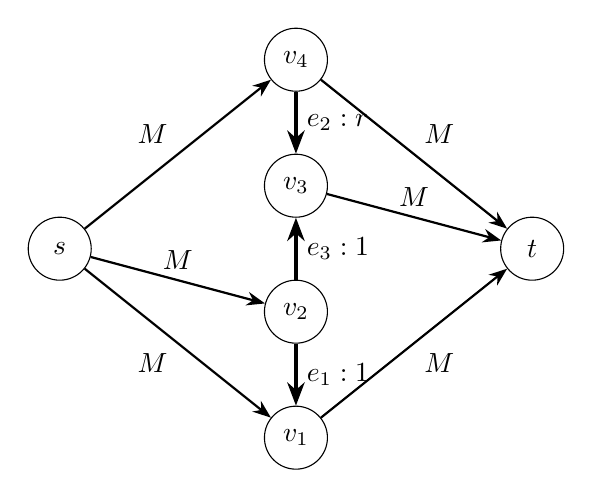
\begin{tikzpicture}[
    >=Stealth,
    vertex/.style={
        circle,
        draw,
        minimum size=8mm,
        inner sep=0pt
    },
    edge/.style={->, thick},
    special/.style={->, very thick}
]

% ------------------------------------------------
% Vertices
% Mapping from top to bottom:
% v4, v3, v2, v1

\node[vertex] (s)  at (-3,0)   {$s$};

\node[vertex] (v4) at (0, 2.4) {$v_4$};
\node[vertex] (v3) at (0, 0.8) {$v_3$};
\node[vertex] (v2) at (0,-0.8) {$v_2$};
\node[vertex] (v1) at (0,-2.4) {$v_1$};

\node[vertex] (t)  at (3,0)    {$t$};

% ------------------------------------------------
% Large-capacity edges

\draw[edge]
    (s) -- node[above left] {$M$} (v4);

\draw[edge]
    (s) -- node[above] {$M$} (v2);

\draw[edge]
    (s) -- node[below left] {$M$} (v1);

\draw[edge]
    (v4) -- node[above right] {$M$} (t);

\draw[edge]
    (v3) -- node[above] {$M$} (t);

\draw[edge]
    (v1) -- node[below right] {$M$} (t);

% ------------------------------------------------
% Special edges

% e2 : v4 -> v3, capacity r
\draw[special]
    (v4) -- node[right] {$e_2:r$} (v3);

% e3 : v2 -> v3, capacity 1
\draw[special]
    (v2) -- node[right] {$e_3:1$} (v3);

% e1 : v2 -> v1, capacity 1
\draw[special]
    (v2) -- node[right] {$e_1:1$} (v1);

\end{tikzpicture}
\end{figure}

\paragraph{Pathological augmenting-path sequence.}

First choose the initial augmenting path
\[
P_0=(s,v_2,v_3,t),
\]
which sends one unit of flow and saturates $e_3$.

Define the following residual augmenting paths:
\begin{align*}
P_1 &= (s,v_4,v_3,v_2,v_1,t),\\
P_2 &= (s,v_2,v_3,v_4,t),\\
P_3 &= (s,v_1,v_2,v_3,t).
\end{align*}

Notice that some edges in these paths are
\emph{reverse residual edges} rather than original edges of $G$.
In particular,
\begin{align*}
P_1 &: \quad v_3 \to v_2
      \text{ is the reverse residual edge of }e_3,\\
P_2 &: \quad v_3 \to v_4
      \text{ is the reverse residual edge of }e_2,\\
P_3 &: \quad v_1 \to v_2
      \text{ is the reverse residual edge of }e_1.
\end{align*}

After $P_0$, repeatedly choose
\[
\boxed{
P_1,\;P_2,\;P_1,\;P_3
}
\]
indefinitely. Thus the complete sequence is
\[
\boxed{
P_0,\;
(P_1,P_2,P_1,P_3),\;
(P_1,P_2,P_1,P_3),\;
(P_1,P_2,P_1,P_3),\ldots
}
\]

If the residual capacities of $(e_1,e_2,e_3)$ are initially
\[
(a_n,a_{n+1},0),
\]
then one four-path cycle gives
\begin{align*}
(a_n,a_{n+1},0)
&\xrightarrow{P_1}
(a_{n+2},0,a_{n+1})\\
&\xrightarrow{P_2}
(a_{n+2},a_{n+1},0)\\
&\xrightarrow{P_1}
(0,a_{n+3},a_{n+2})\\
&\xrightarrow{P_3}
(a_{n+2},a_{n+3},0).
\end{align*}

Here
\[
a_{n+2}=a_n-a_{n+1},
\qquad
a_0=1,
\qquad
a_1=r.
\]

Since
\[
r^2=1-r,
\]
we have
\[
a_n=r^n>0
\]
for every finite $n$. Therefore every cycle leaves another
positive-capacity augmenting path, so Ford--Fulkerson never terminates.




\paragraph{Why the outer arcs never become the bottleneck.}
After the initial augmentation of size 1, the augmentation amounts are
$r,r,r^2,r^2,r^3,r^3,\ldots$. Their total is
$1+2r/(1-r)<5$. Thus every capacity-$M$ outer arc retains forward residual capacity
greater than 1 when $M\ge6$, while every prescribed bottleneck is at most 1.
This validates the entire infinite sequence, not just the recurrence on the three special arcs.


\subsection{Random-endpoint vertex cover: an optional expectation proof}
\label{app:randomvc}
For an unweighted graph, repeatedly choose any uncovered edge and select one of its two
endpoints uniformly at random, then remove all edges incident to the selected vertex.
Return the selected vertices. Each iteration removes at least its chosen edge, and every
removed edge is covered, so the output is feasible.

Fix a minimum cover $C^*$. There are at most $n$ iterations, since selected vertices are
distinct. For each $i\in\{1,\ldots,n\}$, let $A_i$ indicate that iteration $i$ occurs,
and let $Y_i$ indicate that it selects a vertex of $C^*$; after termination set both to zero.
Conditional on the history of any active iteration, the chosen edge has at least one
endpoint in $C^*$, so
\[
\mathbb E[Y_i\mid\text{history}]\ge\tfrac12 A_i.
\]
Taking expectations and summing gives
\[
\tfrac12\mathbb E[|C|]=\tfrac12\sum_i\mathbb E[A_i]
\le\mathbb E\!\left[\sum_iY_i\right]\le |C^*|.
\]
Thus $\mathbb E[|C|]\le2\OPT$. This does not claim a factor-2 bound for every run.
Maintaining active edges and removing a vertex's incident edges gives polynomial time.
The simpler maximal-matching algorithm in the main notes is deterministic and has the
same approximation factor.

\end{multicols*}

\end{document}
